% Copyright 2004 by Till Tantau <tantau@users.sourceforge.net>.
%
% In principle, this file can be redistributed and/or modified under
% the terms of the GNU Public License, version 2.
%
% However, this file is supposed to be a template to be modified
% for your own needs. For this reason, if you use this file as a
% template and not specifically distribute it as part of a another
% package/program, I grant the extra permission to freely copy and
% modify this file as you see fit and even to delete this copyright
% notice. 
\documentclass{beamer}
\usepackage{bbm}
\usepackage{lipsum}
\usepackage{enumitem}
\usepackage{pifont}
\usepackage{tikz}
\usepackage{lmodern}
\usepackage{commath}
\usepackage{bbm} %package for using the bbm fonts in math environment
\usetikzlibrary{calc}
\usepackage{xparse} 
\usetikzlibrary{calc}
\logo{\color{red}\rule{.5cm}{.5cm}}
\newcommand{\btVFill}{\vskip0pt plus 1filll}
\usepackage{afterpage}
\usepackage{xcolor}

%\usepackage{xcolor}
%\usepackage{tikz}
%\usetikzlibrary{shadows}
\newlength{\tmpShadow}
\newcommand{\MyShadow}[2]{%
	\settowidth{\tmpShadow}{#1}
	\addtolength{\tmpShadow}{.1em}
	\raisebox{-0.25ex}{\textcolor{gray!70}{#1}}%
	\kern-\tmpShadow%
	\textcolor{#2}{#1}%
}


\tikzset{
	invisible/.style={opacity=0,text opacity=0},
	visible on/.style={alt=#1{}{invisible}},
	alt/.code args={<#1>#2#3}{%
		\alt<#1>{\pgfkeysalso{#2}}{\pgfkeysalso{#3}} 
	},
}
\tikzset{
	background fill/.style={fill=#1},
	background fill/.default={white},
	fill on/.style={alt=#1{}{background fill}},
}
\tikzset{
	background draw/.style={draw=#1},
	background draw/.default={white},
	draw on/.style={alt=#1{}{background draw}},
}
\tikzset{
	background filldraw/.style args={#1 filled by #2}{draw=#1, fill=#2},
	background filldraw/.default=white filled by white,
	filldraw on/.style={alt=#1{}{background filldraw}},
}
\tikzset{highlighting/.style={
		append after command={
			\pgfextra{
				\path[rounded corners,
				background draw=red,
				draw on=<#1>,
				overlay] ($(\tikzlastnode.south west)+(-0.015,-0.1)$) % to have some offset
				rectangle ($(\tikzlastnode.north east)+(0.015,0.07)$);
			}   
		}
	}
}
\NewDocumentCommand{\highlight}{r<> m}{%
	\tikz[baseline=(A.base)] 
	\node[highlighting=#1,
	inner sep=0pt] (A) {#2};%
}

%\newcommand*{\MyShadowBullet}{\tikz \draw [baseline, fill=blue,draw=blue,circular drop shadow] circle (2pt);}
%\newcommand*{\MyBallBullet}{\tikz \draw [baseline, ball color=red, draw=red] circle (2pt);}

\newcommand{\nologo}{\setbeamertemplate{logo}{}} % command to set the logo to nothing
\usepackage{multicol}
\newcommand\tab[1][1cm]{\hspace*{#1}}

%gets rid of bottom navigation bars
%\setbeamertemplate{footline}[frame number]{}
%gets rid of bottom navigation symbols
\setbeamertemplate{navigation symbols}{}
%gets rid of footer
%will override 'frame number' instruction above
%comment out to revert to previous/default definitions
%\setbeamertemplate{footline}{}

\newcounter{mycounter}  
\newenvironment{noindlist}
{\begin{list}{}{\usecounter{mycounter} \labelsep=0em \labelwidth=0em \leftmargin=0em \itemindent=0em}}
	{\end{list}}

% There are many different themes available for Beamer. A comprehensive
% list with examples is given here:
% http://deic.uab.es/~iblanes/beamer_gallery/index_by_theme.html
% You can uncomment the themes below if you would like to use a different
% one:
%\usetheme{AnnArbor}
%\usetheme{Antibes}
%\usetheme{Bergen}
%\usetheme{Berkeley}
%\usetheme{Berlin}
%\usetheme{Boadilla}
%\usetheme{boxes}
%\usetheme{CambridgeUS}
%\usetheme{Copenhagen}
%\usetheme{Darmstadt}
%\usetheme{default}
%\usetheme{Frankfurt}
%\usetheme{Goettingen}
%\usetheme{Hannover}
%\usetheme{Ilmenau}
%\usetheme{JuanLesPins}
%\usetheme{Luebeck}
\usetheme{Madrid}
%\usetheme{Malmoe}
%\usetheme{Marburg}
%\usetheme{Montpellier}
%\usetheme{PaloAlto}
%\usetheme{Pittsburgh}
%\usetheme{Rochester}
%\usetheme{Singapore}
%\usetheme{Szeged}
%\usetheme{Warsaw}

%\setbeamercolor{normal text}{fg=white,bg=black!90}
%\setbeamercolor{structure}{fg=blue!80}
%\setbeamercolor{alerted text}{fg=red!85!black}
%\setbeamercolor{item projected}{use=item,fg=black,bg=item.fg!35}
%\setbeamercolor*{palette primary}{use=structure,fg=structure.fg}
%\setbeamercolor*{palette secondary}{use=structure,fg=structure.fg!95!black}
%\setbeamercolor*{palette tertiary}{use=structure,fg=structure.fg!90!black}
%\setbeamercolor*{palette quaternary}{use=structure,fg=structure.fg!95!black,bg=black!80}
%\setbeamercolor*{framesubtitle}{fg=white}
%\setbeamercolor*{block title}{parent=structure,bg=black!60}
%\setbeamercolor*{block body}{fg=black,bg=blue!10}
%\setbeamercolor*{block title alerted}{parent=alerted text,bg=black!15}
%\setbeamercolor*{block title example}{parent=example text,bg=black!15}


\title{Path analysis and feature extraction}

% A subtitle is optional and this may be deleted
%\subtitle{Optional Subtitle}

\author{Avgoustinos~Vouros\inst{1}}
% - Give the names in the same order as the appear in the paper.
% - Use the \inst{?} command only if the authors have different
%   affiliation.

\institute[] % (optional, but mostly needed)
{
  \inst{1}%
  PhD student, \\Department of Computer Science,\\
  University of Sheffield\\
  \vspace{5mm}
  \noindent Supervised by Prof Eleni Vasilaki
  %\and
  %\inst{2}%
  %Department of Theoretical Philosophy\\
  %University of Elsewhere
}

\date{} %removes the date
% - Use the \inst command only if there are several affiliations.
% - Keep it simple, no one is interested in your street address.

%\date{Conference Name, 2013}
% - Either use conference name or its abbreviation.
% - Not really informative to the audience, more for people (including
%   yourself) who are reading the slides online

%\subject{Theoretical Computer Science}
% This is only inserted into the PDF information catalog. Can be left
% out. 

% If you have a file called "university-logo-filename.xxx", where xxx
% is a graphic format that can be processed by latex or pdflatex,
% resp., then you can add a logo as follows:

\pgfdeclareimage[height=1cm]{university-logo}{university-logo}
\logo{\pgfuseimage{university-logo}}

% Delete this, if you do not want the table of contents to pop up at
% the beginning of each subsection:
\AtBeginSubsection[]
{
  \begin{frame}<beamer>{Outline}
    \tableofcontents[]
  \end{frame}
}

% Let's get started
\begin{document}

\begin{frame}
  \titlepage
\end{frame}

%\begin{frame}{Acknowledgements}
%	Original slides created by: 
%	\begin{itemize}
%		\item Eleni Vasilaki (Prof)
%		\item Tiago V. Gehring (PhD)
%	\end{itemize}
%	\vspace{5mm}
%	Revised and modified slides created by:
%	\begin{itemize}
%		\item Avgoustinos Vouros
%	\end{itemize}	
%\end{frame}

%%%%%%%%%%%%%%%%%%%%%%%%%%%%%%%%%%%%%%%%%%%%%%%%%%%%%%%%%

%\begin{frame}{Contents}
%	\begin{itemize}[label={\MyShadow{$\bullet$}{black!80}}]
%		\item The story so far...
%		\vspace{3mm}
%		\item Features
%		\vspace{3mm}
%		\begin{itemize}[label={\MyShadow{$\bullet$}{black!80}}]
%			\item Theory
%			\begin{itemize}[label={\MyShadow{$\star$}{black!80}}]
%				\item Regression (quick)
%			\end{itemize}	
%			\vspace{3mm}
%			\item Algorithm
%			\vspace{3mm}
%			\item Tuning
%			\begin{itemize}[label={\MyShadow{$\star$}{black!80}}]
%				\item Gap Statistic
%			\end{itemize}				
%		\end{itemize}
%		\vspace{1mm}
%		\item Ongoing Research
%	\end{itemize}
%\end{frame}


\begin{frame}[plain,c]
%\frametitle{A first slide}
	\vspace{1mm}
	\begin{center}
		\Huge The story so far...
	\end{center}
\end{frame}

{\nologo
\begin{frame}{The story so far...}
\begin{multicols}{2}
	\begin{itemize}
		\item<1->
		\begin{figure}[H]
			\centering
			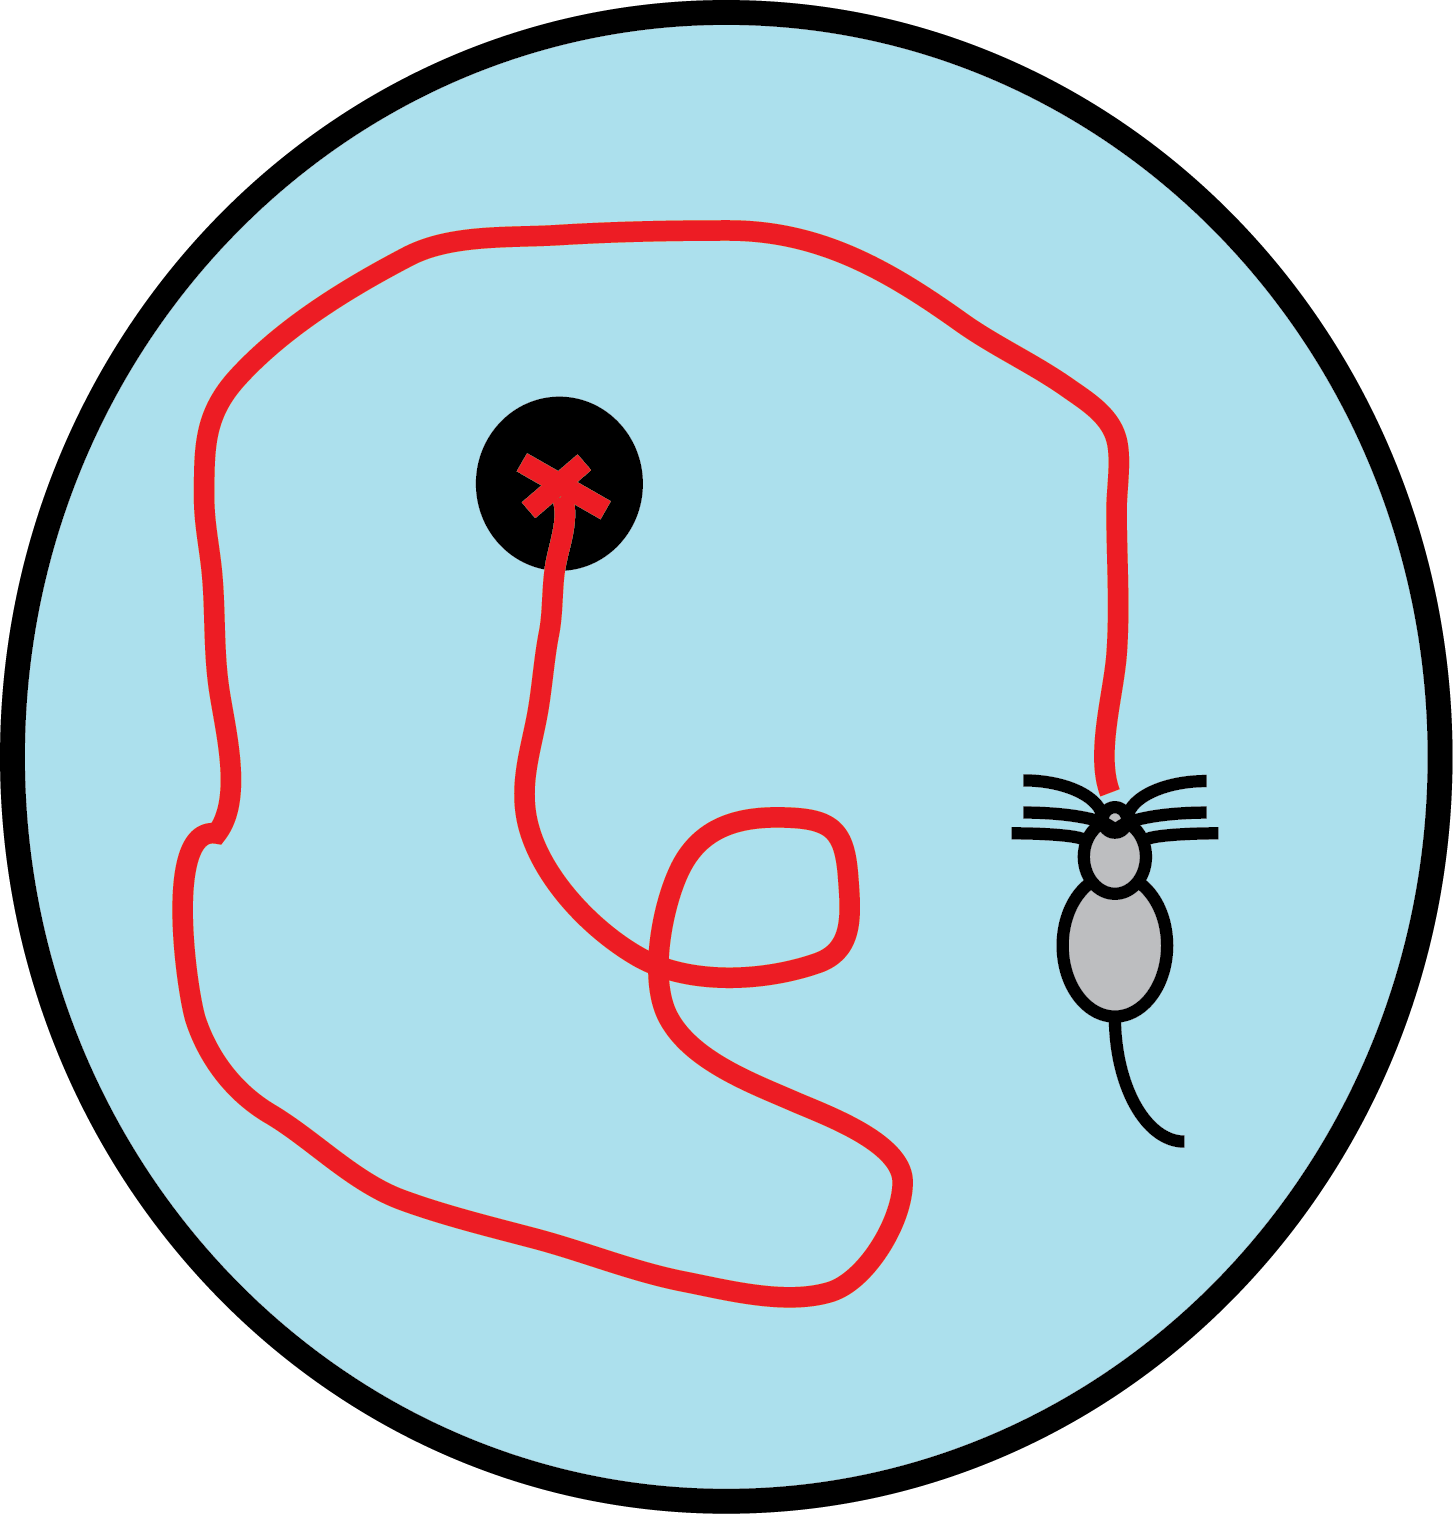
\includegraphics[width=0.3\textwidth]{figures/MWM}
		\end{figure}
		\vspace{5mm}
		\item<2->
		\begin{figure}[H]
			\centering
			
\includegraphics[width=0.3\textwidth]{figures/perfM}
		\end{figure}	
		\vspace{5mm}
		\item<3->
		\begin{figure}[H]
			\centering
			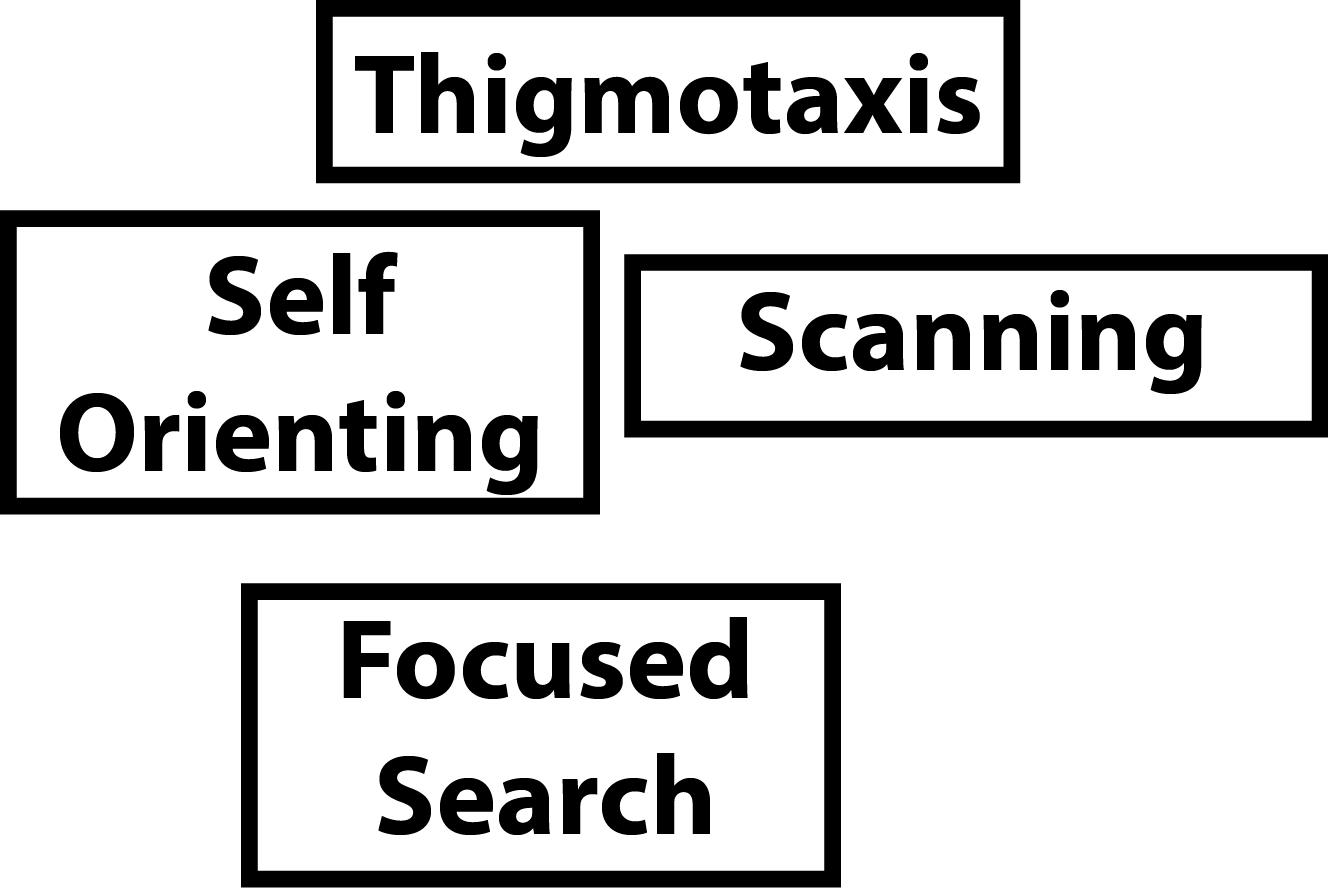
\includegraphics[width=0.3\textwidth]{figures/labels}
		\end{figure}	
		\vspace{4mm}
		\item<4->
		\begin{figure}[H]
			\centering
			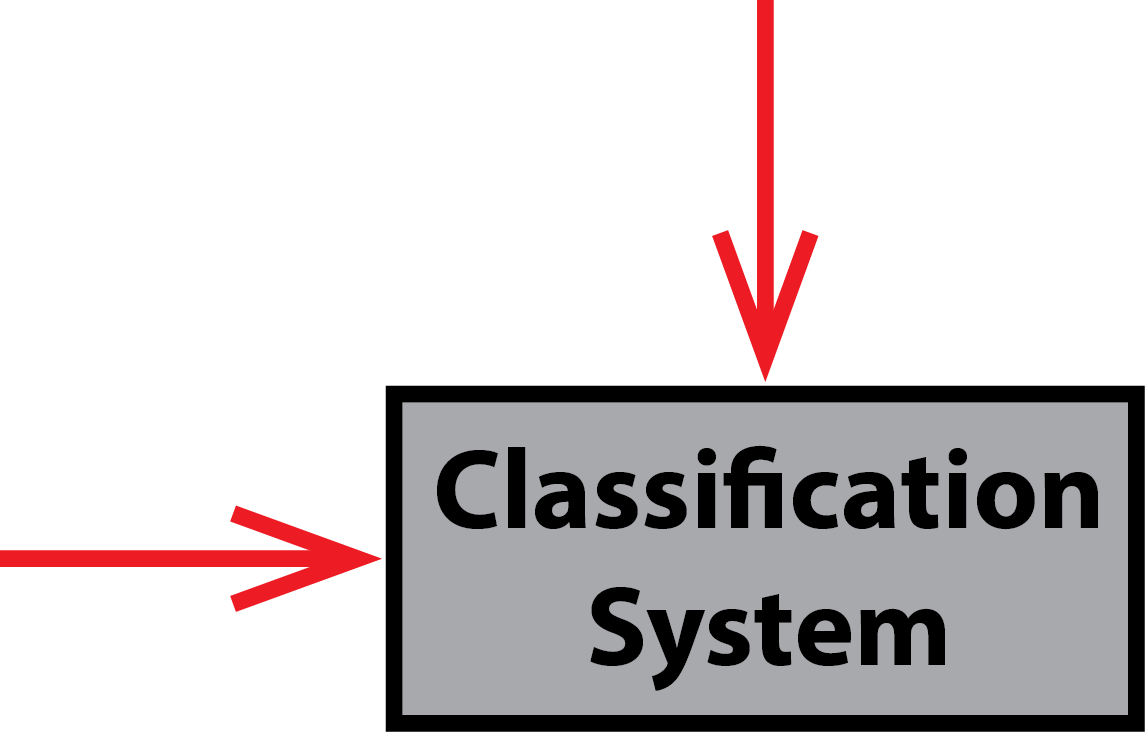
\includegraphics[width=0.3\textwidth]{figures/classifier}
		\end{figure}		
	\end{itemize}
\end{multicols}	
\end{frame}

\begin{frame}{The story so far...}
\begin{multicols}{2}
	\begin{itemize}
		\item<1->
		\begin{figure}[H]
			\centering
			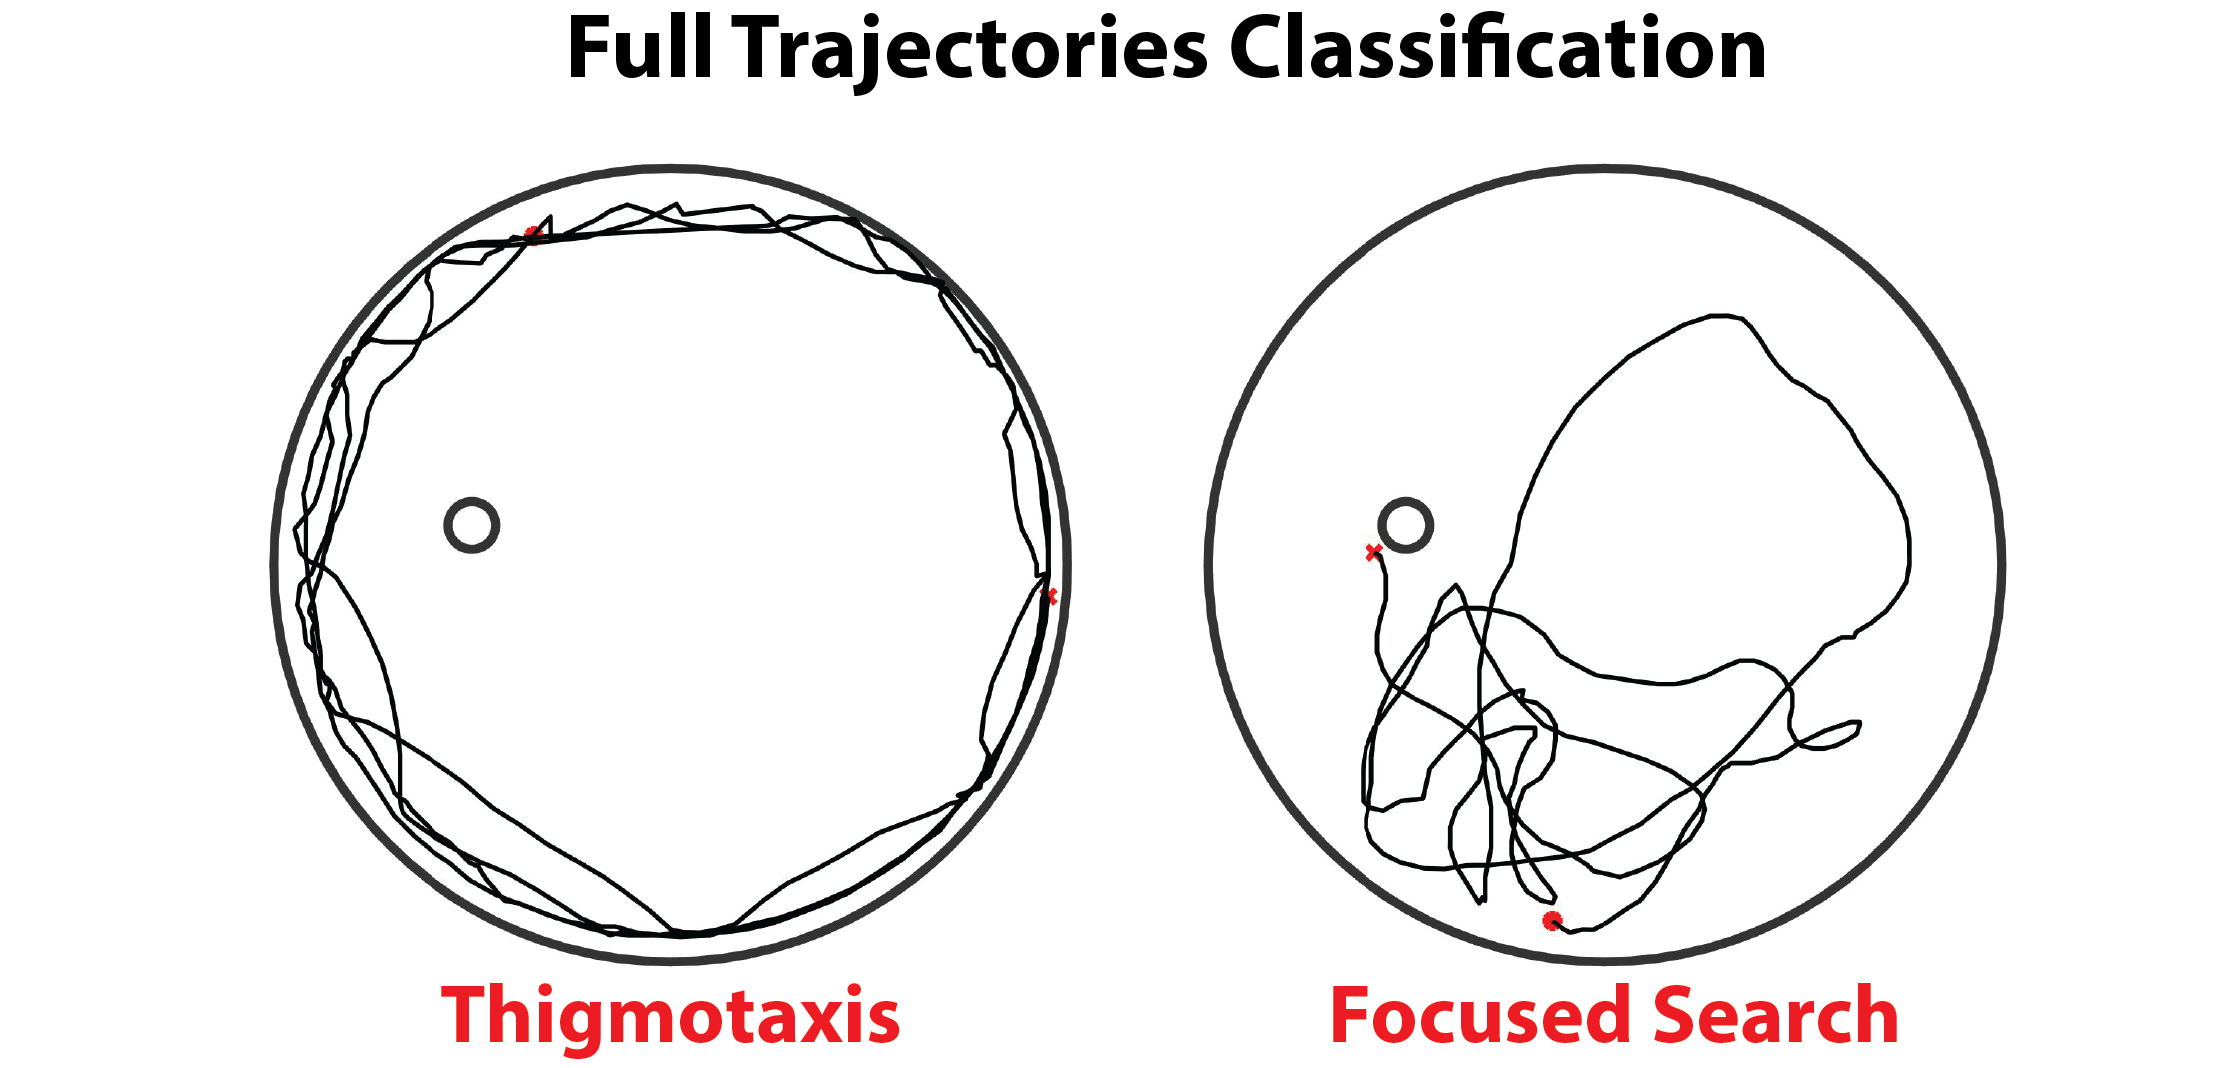
\includegraphics[width=0.57\textwidth]{figures/others}
		\end{figure}	
		\vspace{4mm}	
		\item<2->
		\small{
		\begin{itemize}[label={\MyShadow{$\bullet$}{blue!80}}]
			\item Dalm, S., Grootendorst, J., De Kloet, E. R. (2000).
			\vspace{1.2mm}	
			\item Wolfer, D. P. \& Lipp, H.-P. (2000).
			\vspace{1.2mm}
			\item Wolfer, D. P., Madani, R., Valenti, P. \& Lipp, H.-P. (2001).
			\vspace{1.2mm}
			\item Graziano, A., Petrosini, L. \& Bartoletti, A. (2003)
			\vspace{1.2mm}
			\item Illouz, T., Madar, R., Louzon, Y., Griffioen, K. J. \& Okun, E. (2016).
			\vspace{1.2mm}
			\item Rogers, Jake, et al. (2017).
			\vspace{1.2mm}
			\item Higaki, Akinori, et al. (2018).
		\end{itemize}	
		}	
	\end{itemize}
\end{multicols}	
\end{frame}

\begin{frame}{The story so far...}
	\begin{figure}[H]
		\centering
		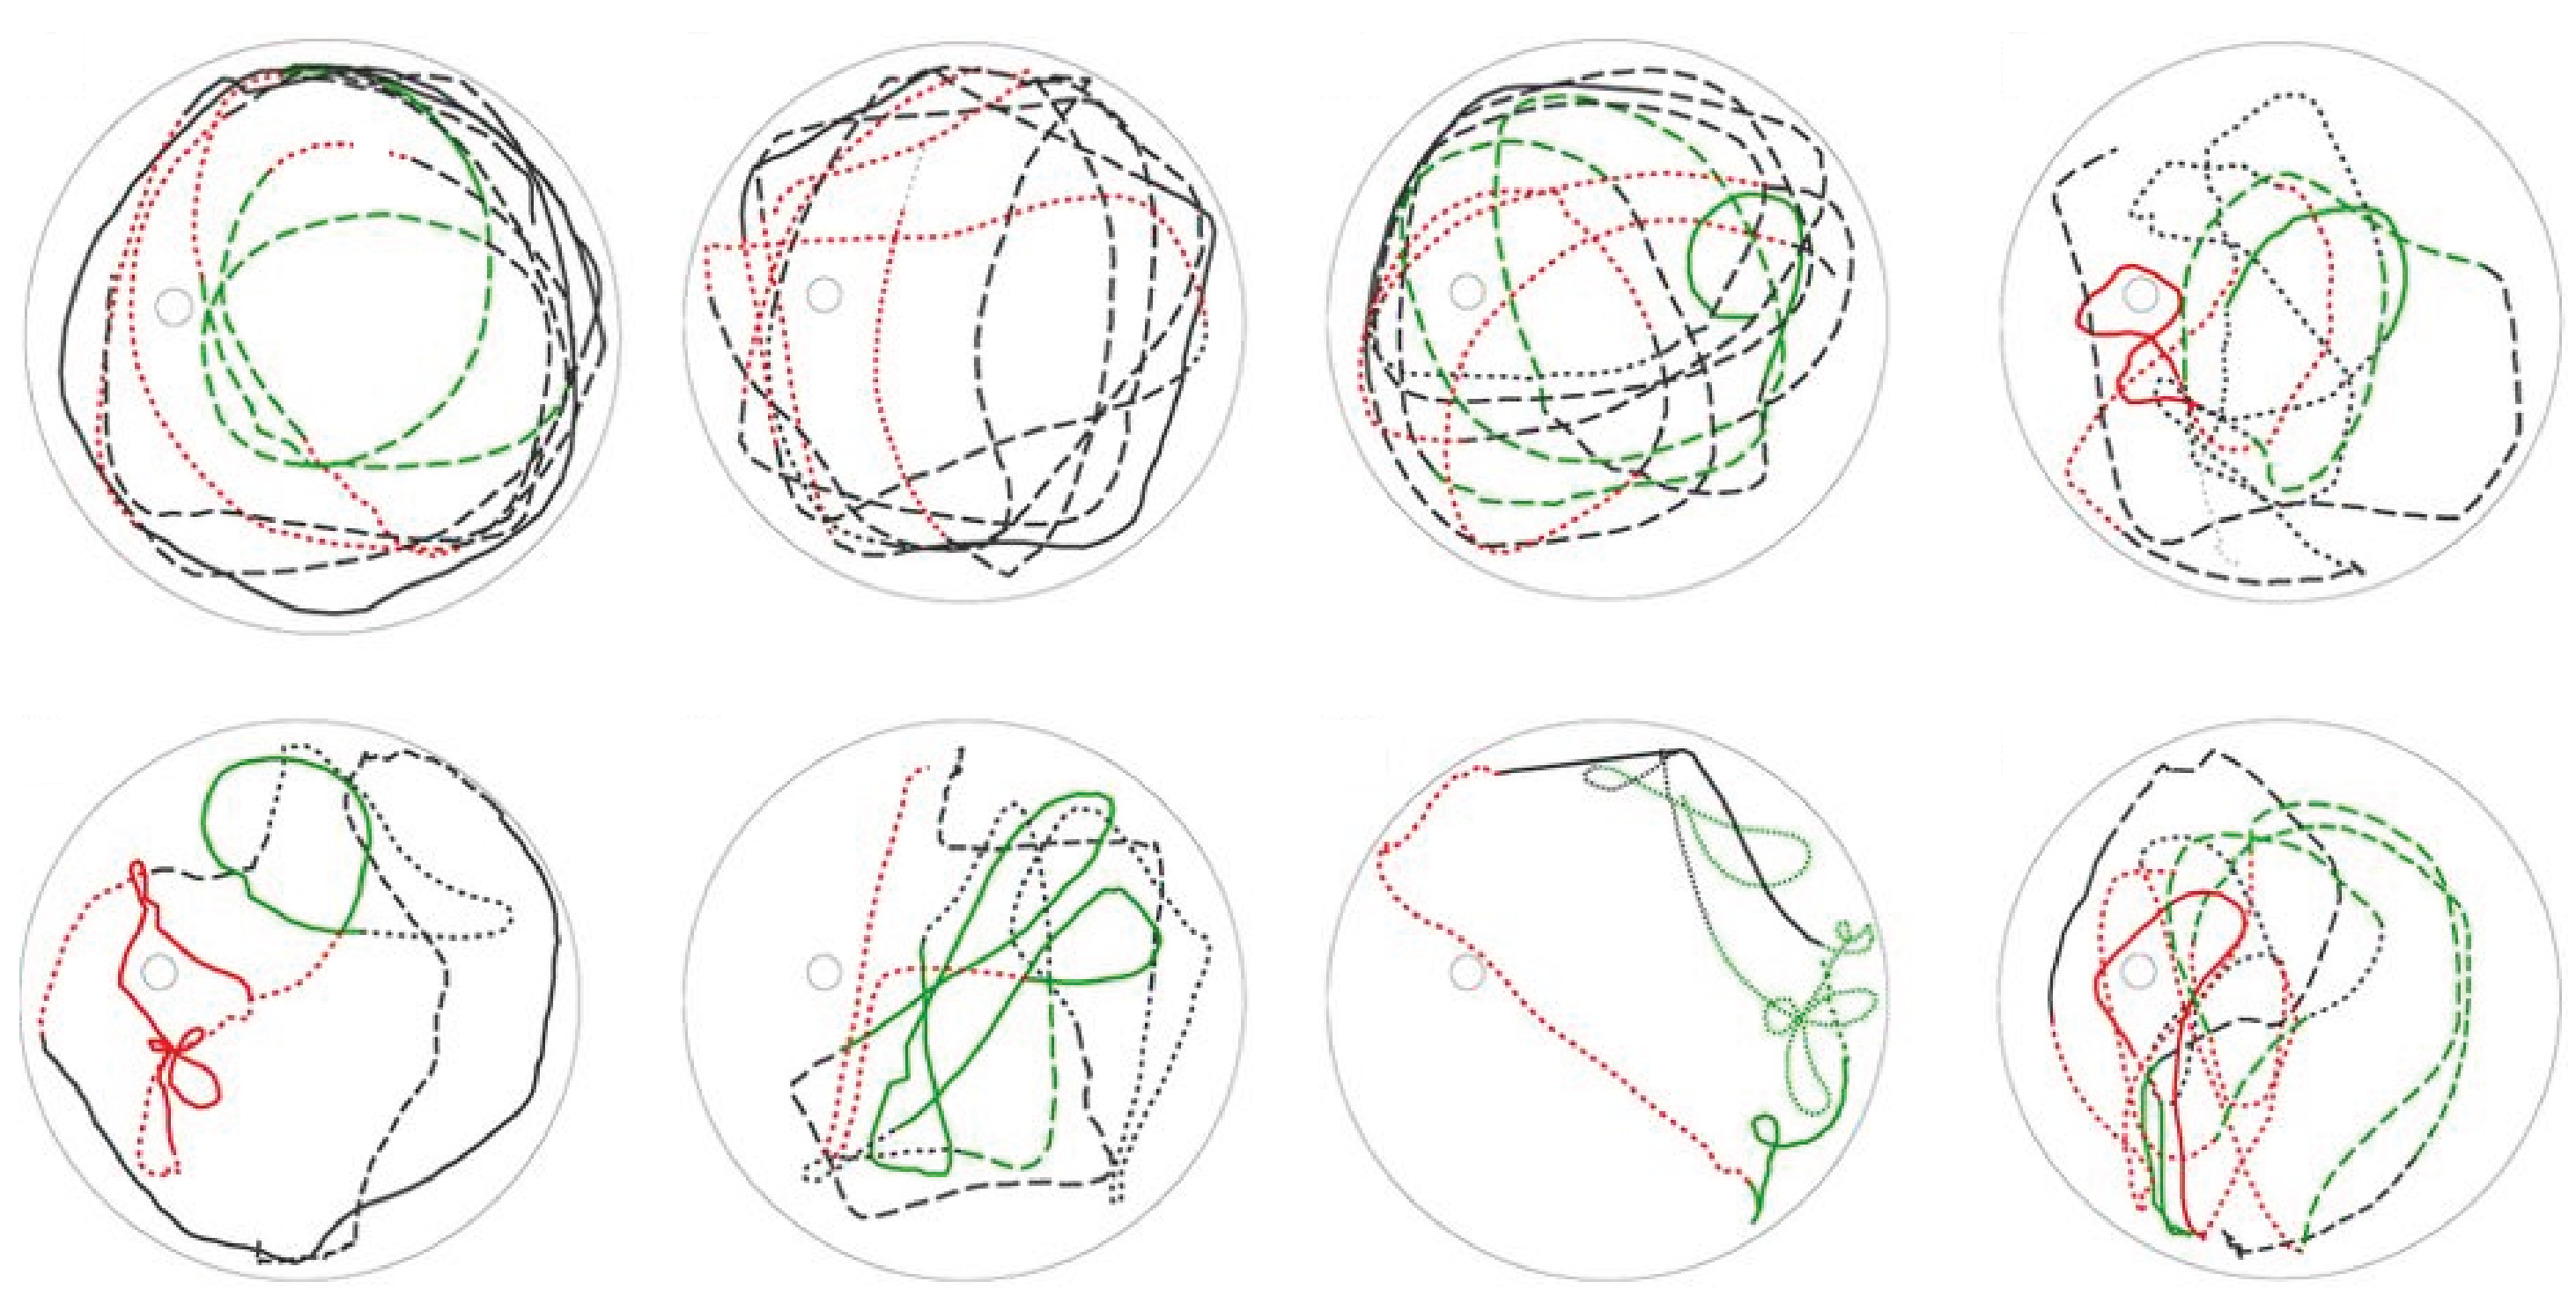
\includegraphics[width=\textwidth]{figures/gehringetal}
	\end{figure}
	\vspace{4mm}
	\tiny{Gehring, Tiago V., et al. "Detailed classification of swimming paths in the Morris Water Maze: multiple strategies within one trial." Scientific reports 5 (2015): 14562.}		
\end{frame}

\begin{frame}{The story so far...}
	\begin{figure}[H]
		\centering
		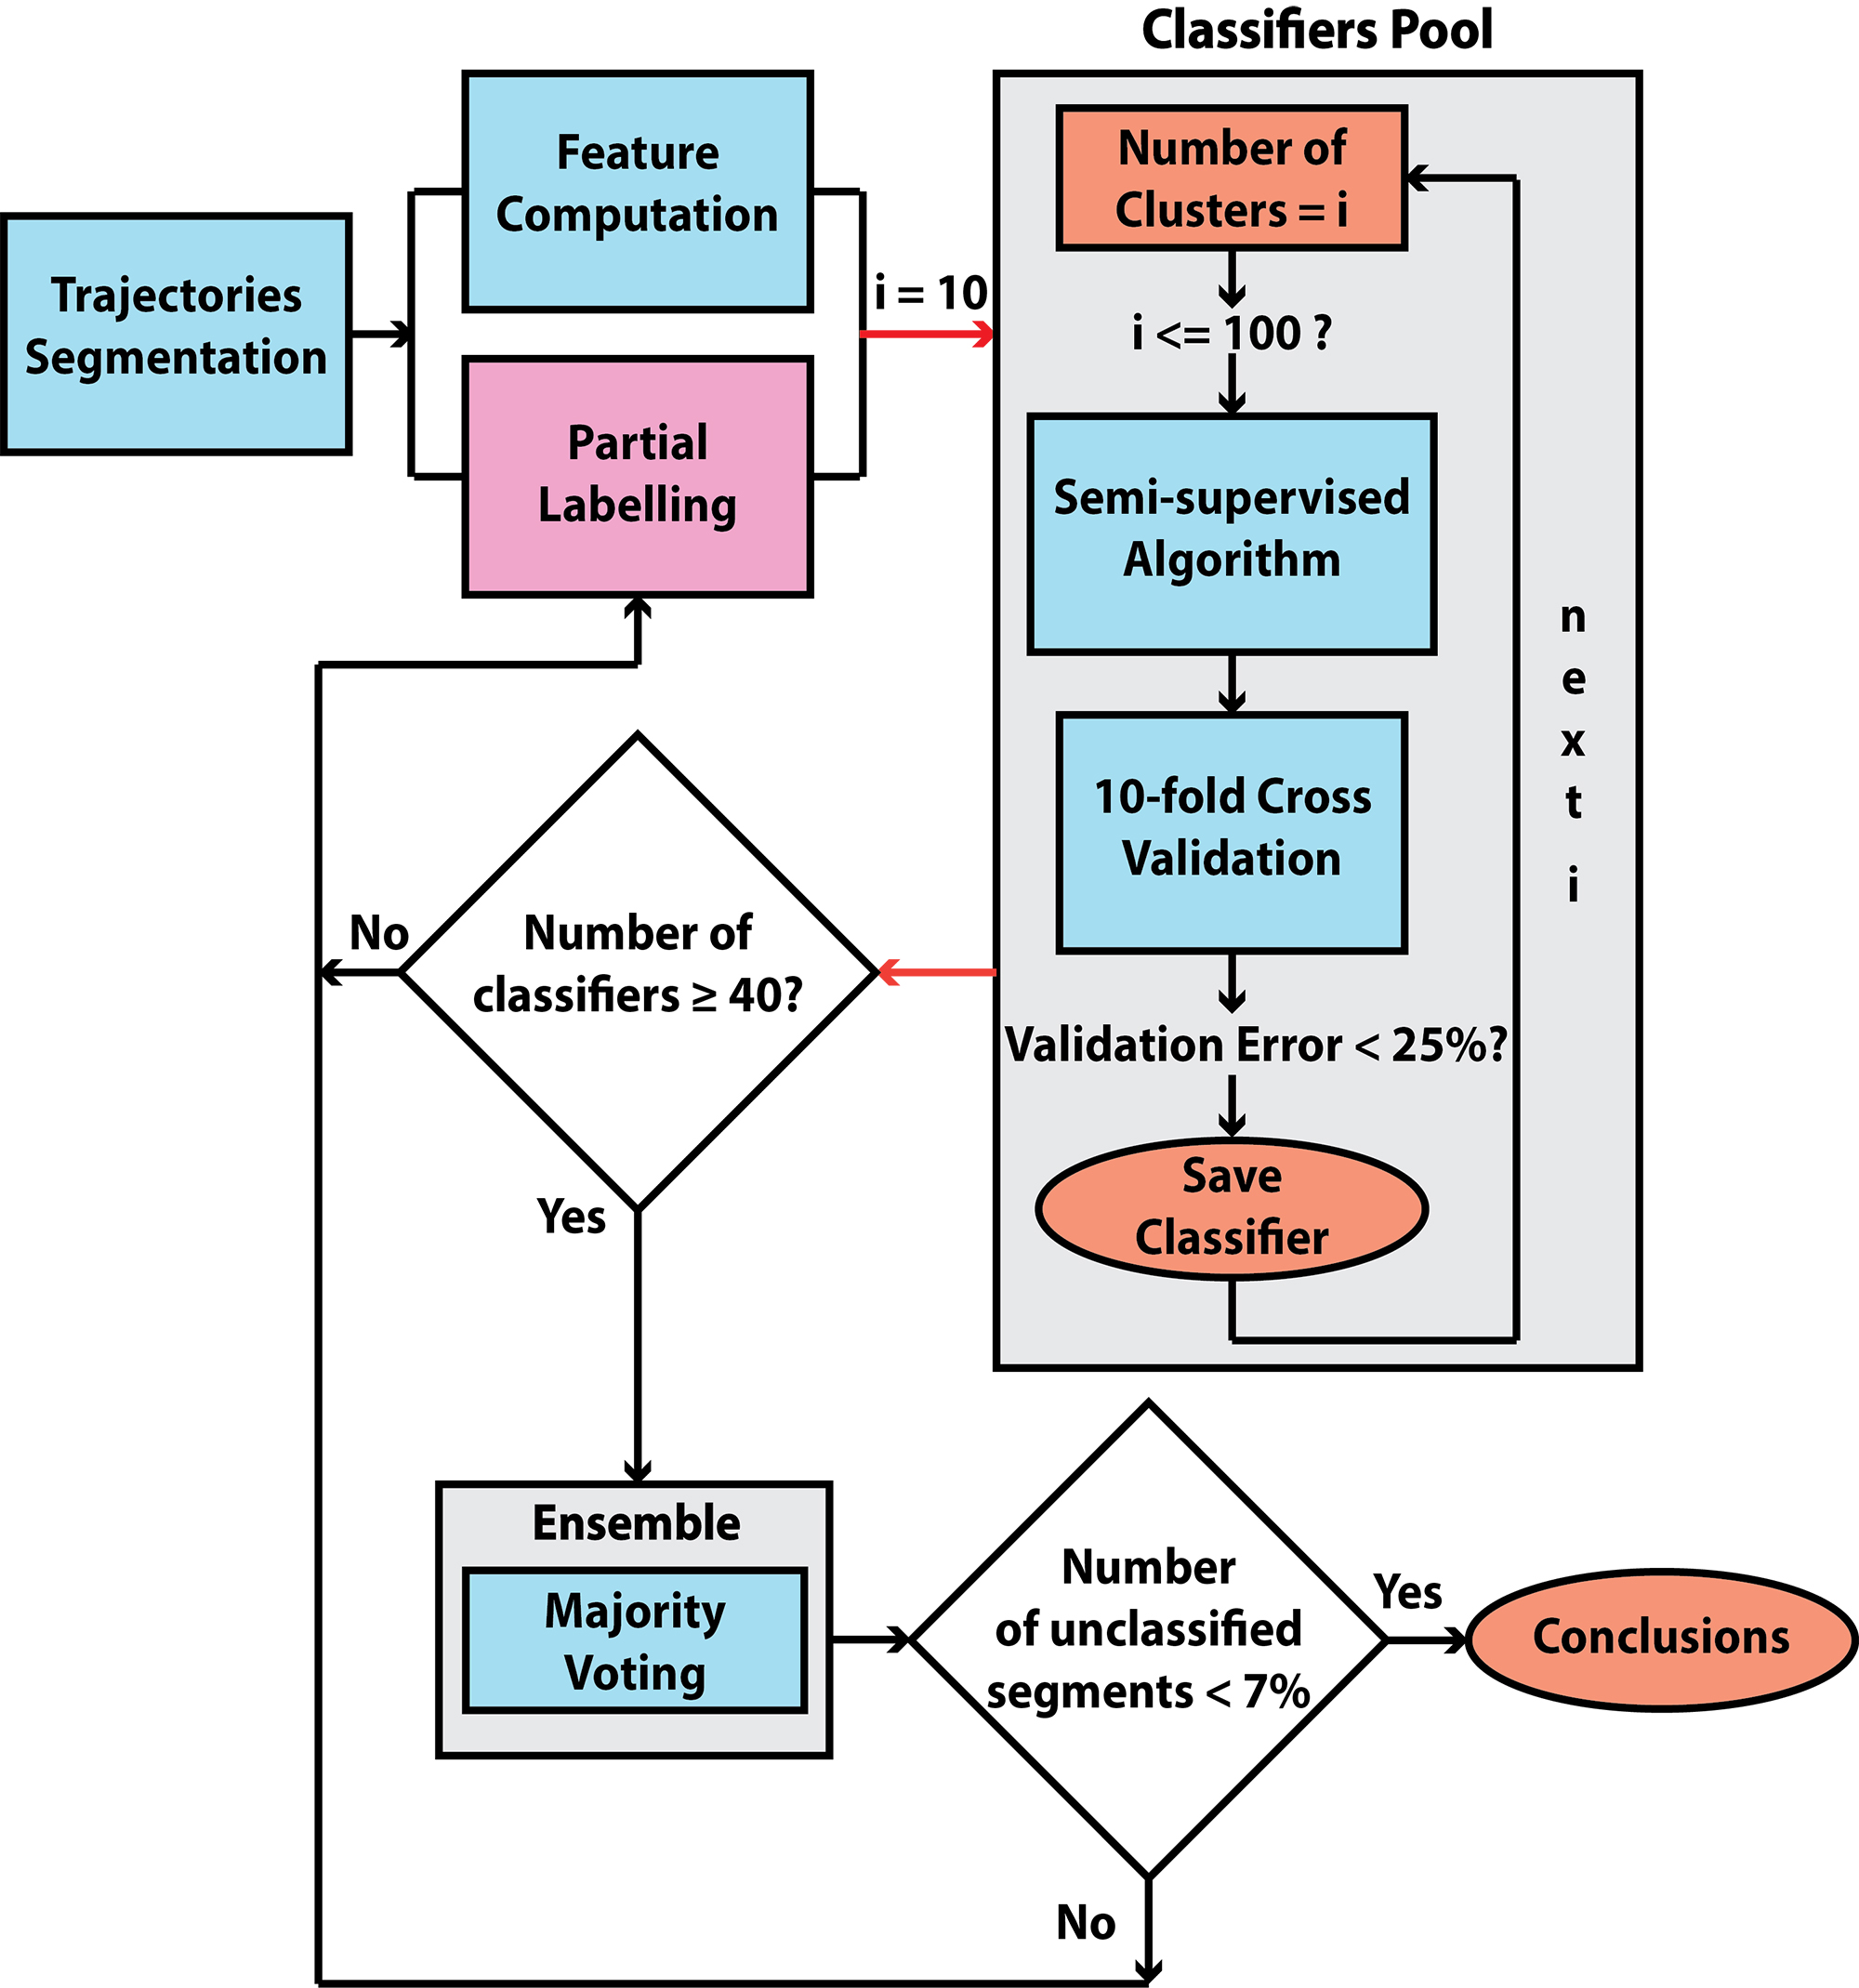
\includegraphics[width=0.56\textwidth]{figures/vourosetal}
	\end{figure}
	\tiny{Vouros, Avgoustinos, et al. "A generalised framework for detailed classification of swimming paths inside the Morris Water Maze." Scientific reports 8.1 (2018): 15089.}		
\end{frame}

\begin{frame}{What about the path features?}
	\begin{multicols}{2}
	\begin{figure}[H]
		\centering
		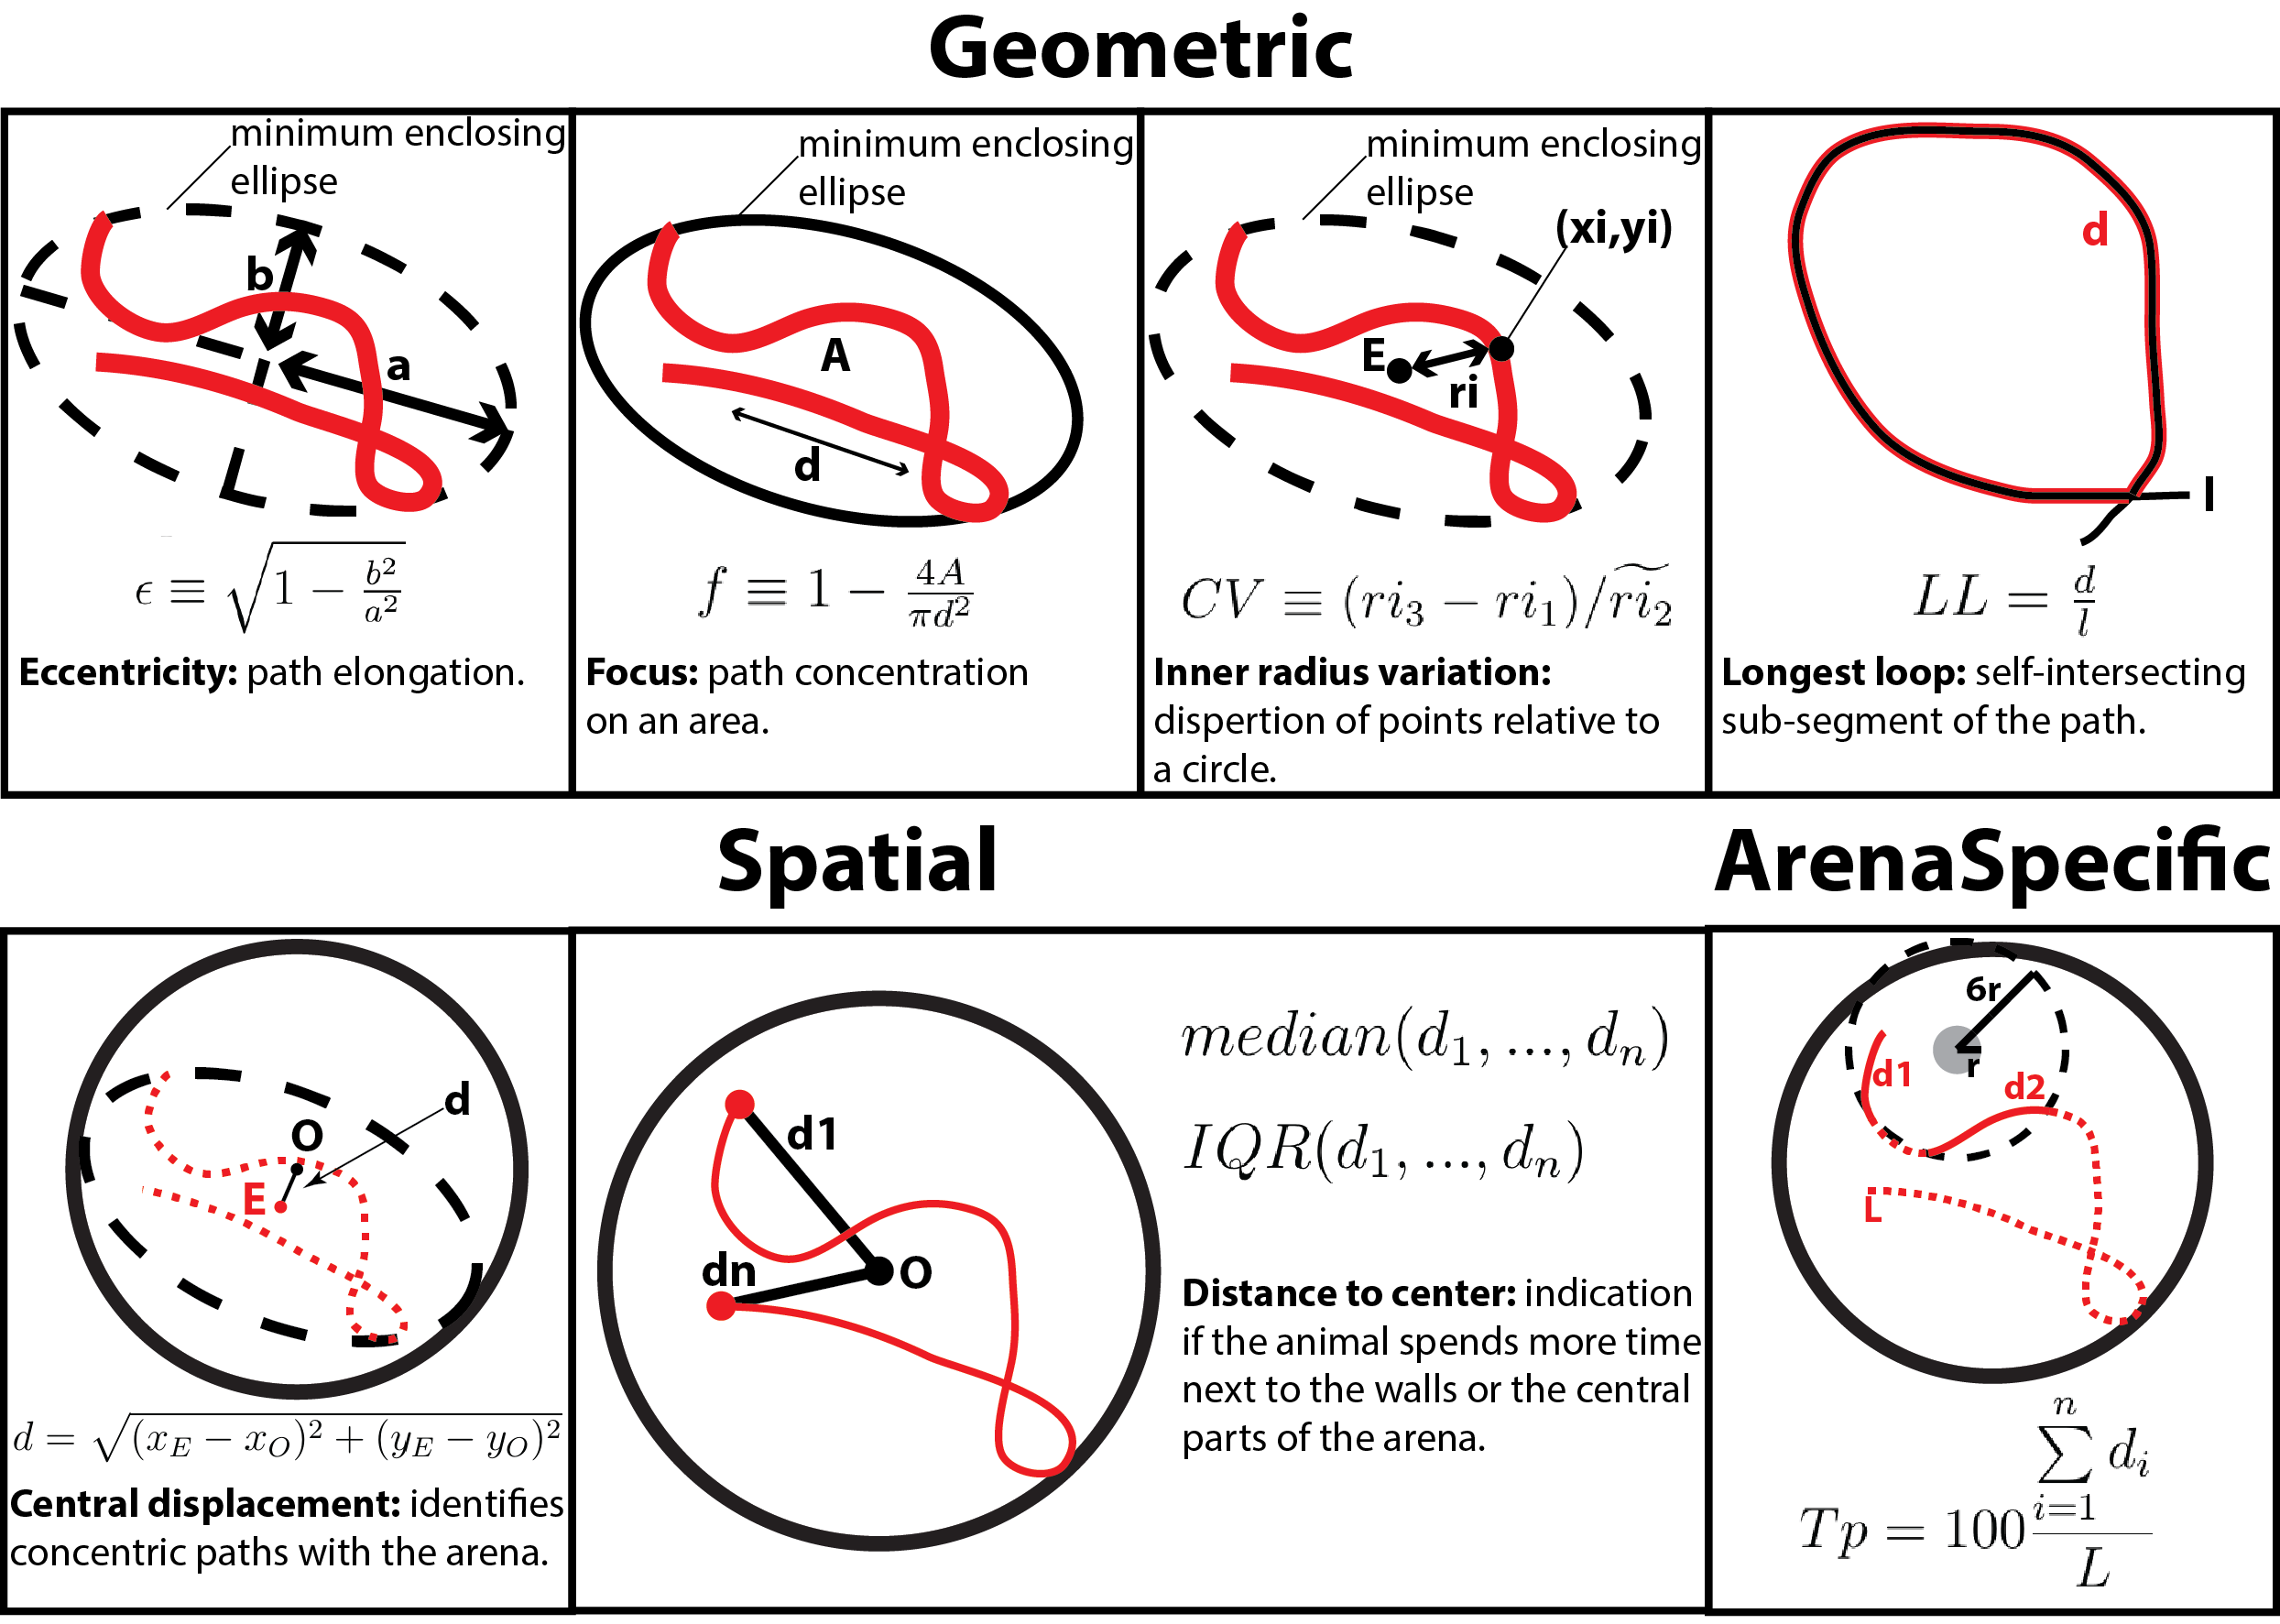
\includegraphics[width=0.8\textwidth]{figures/features}
	\end{figure}
	\tiny{Gehring, Tiago V., et al. "Detailed classification of swimming paths in the Morris Water Maze: multiple strategies within one trial." Scientific reports 5 (2015): 14562.}	
	\end{multicols}	
\end{frame}

\begin{frame}{What about the path features?}
	\begin{figure}[H]
		\centering
		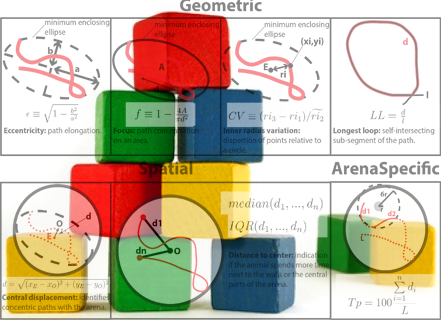
\includegraphics[width=0.8\textwidth]{figures/buildingblocks2}
	\end{figure}
\end{frame}

\begin{frame}{Different experimental procedures}
	\begin{figure}[H]
		\centering
		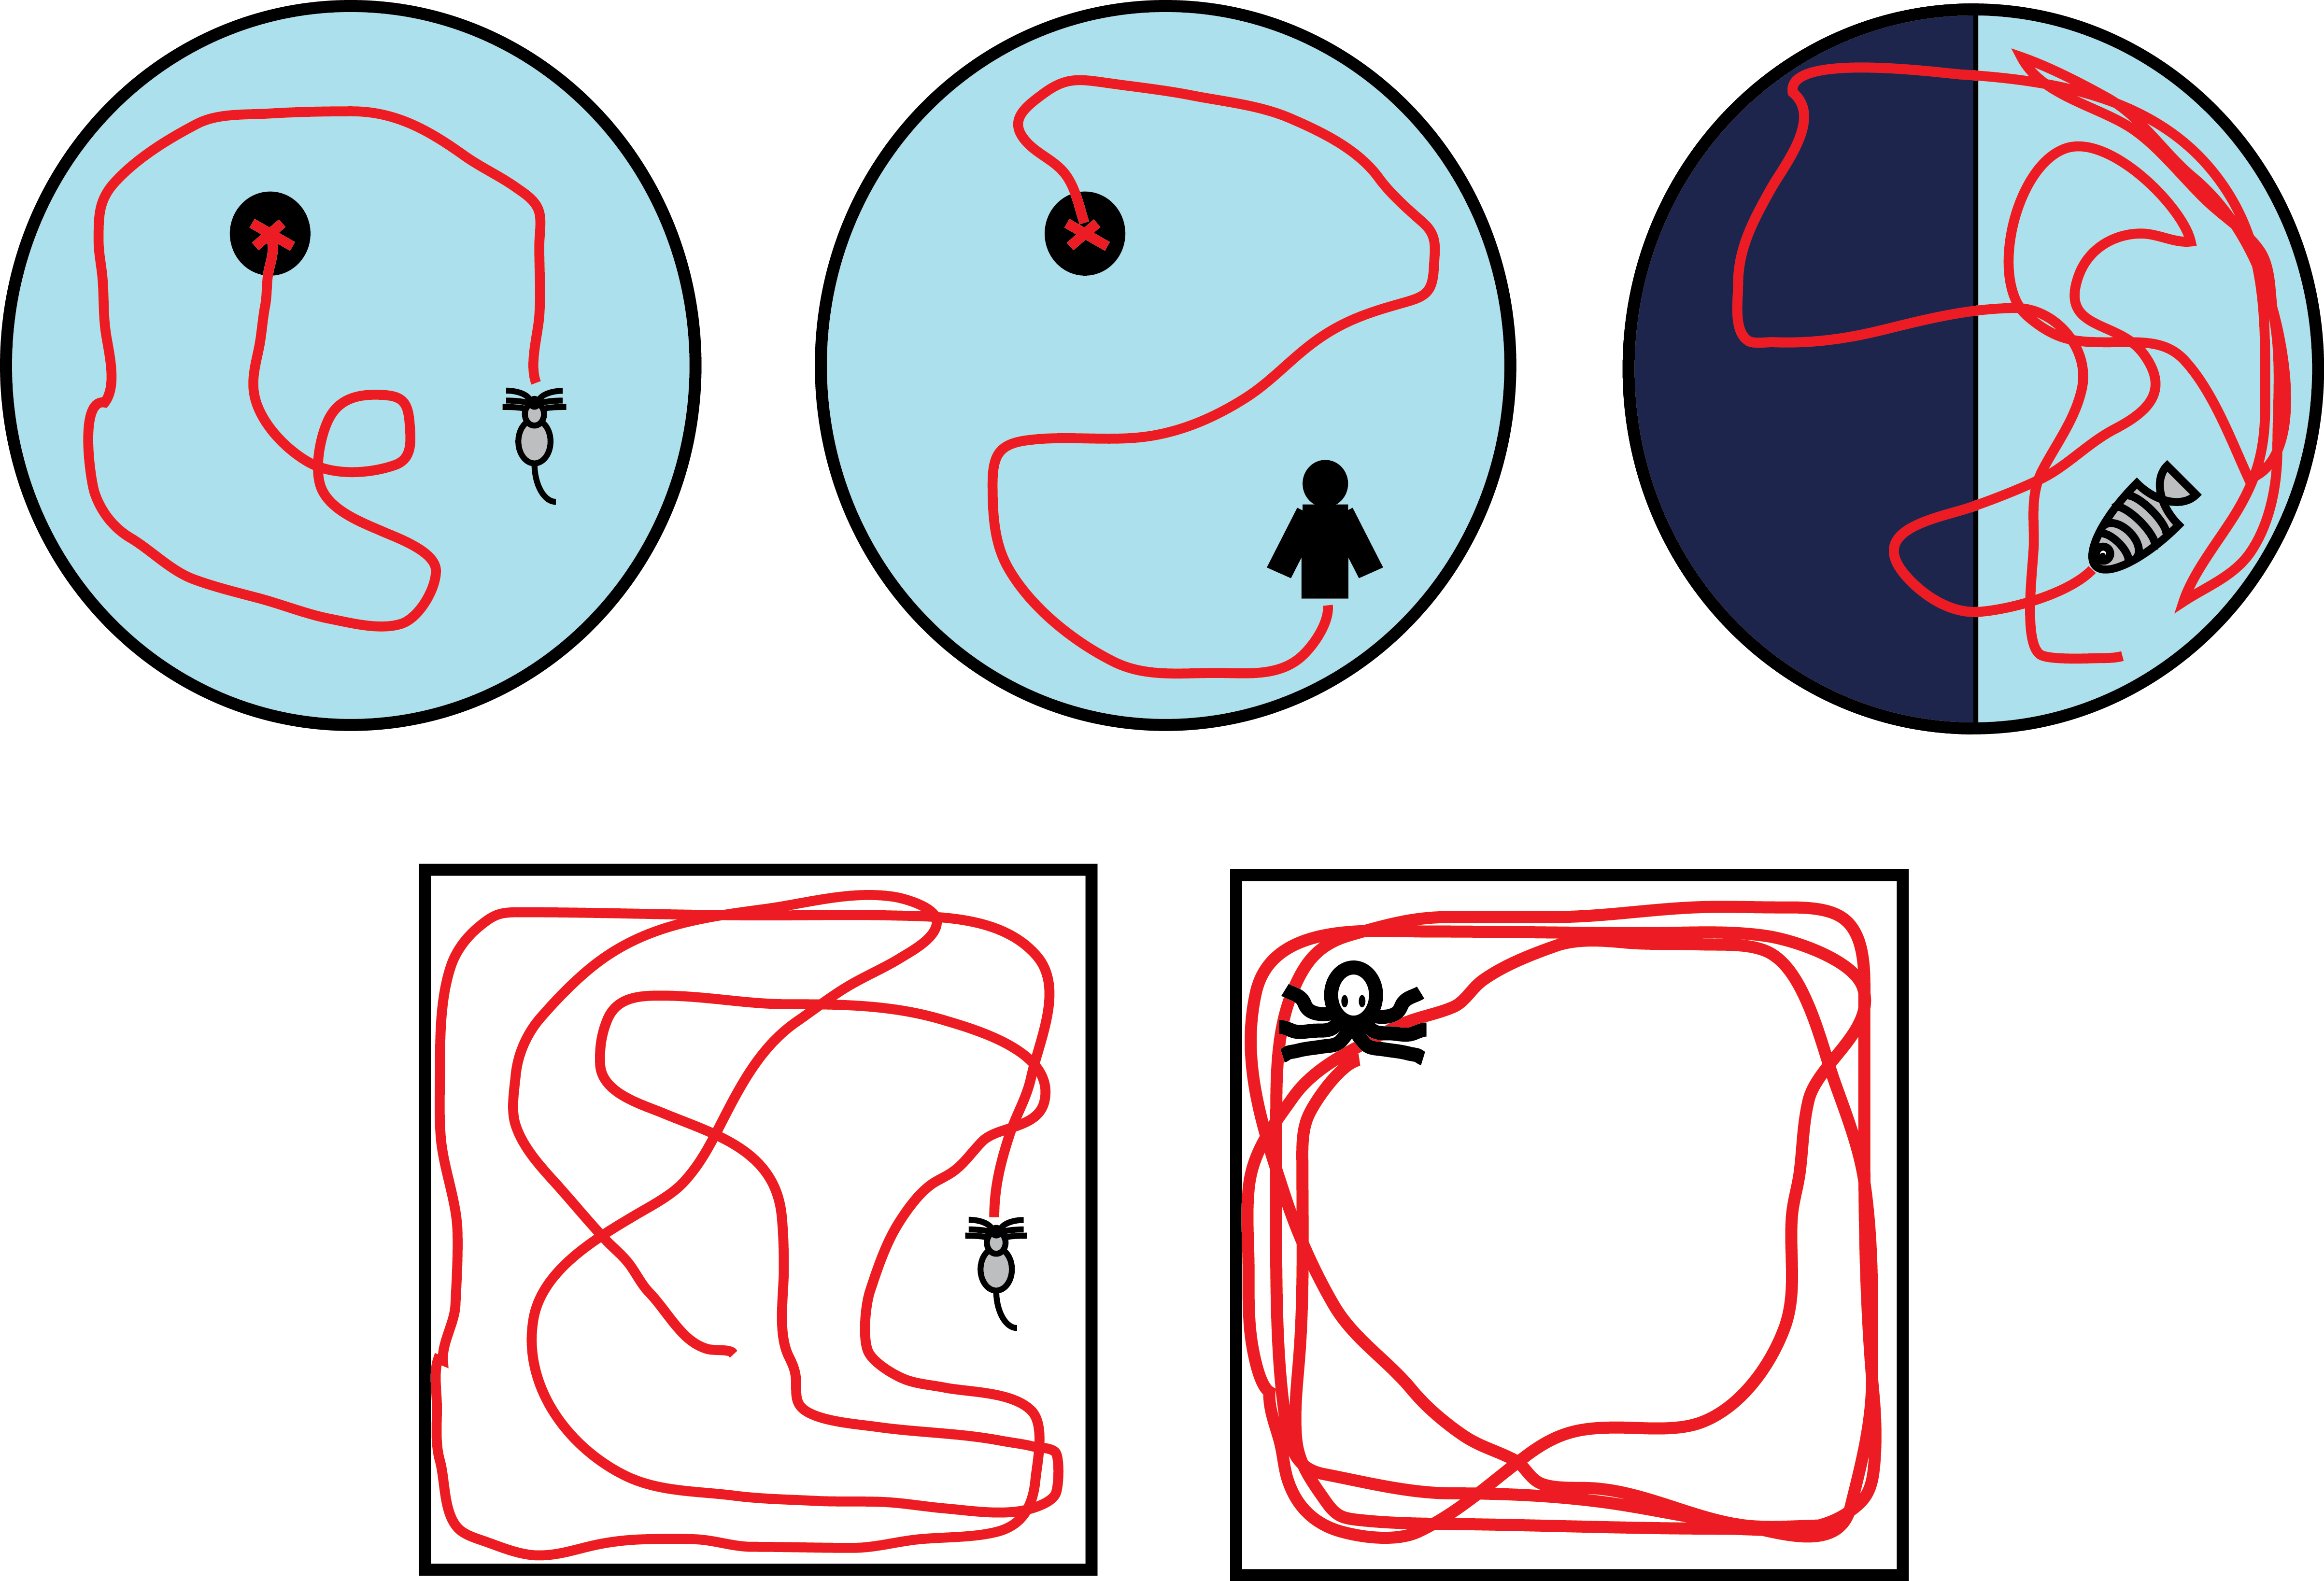
\includegraphics[width=0.95\textwidth]{figures/experiments}
	\end{figure}
\end{frame}
          
\begin{frame}{Why don't we just apply the same frameworks?}
\begin{figure}
	\begin{overprint}
		\onslide<1>\centerline{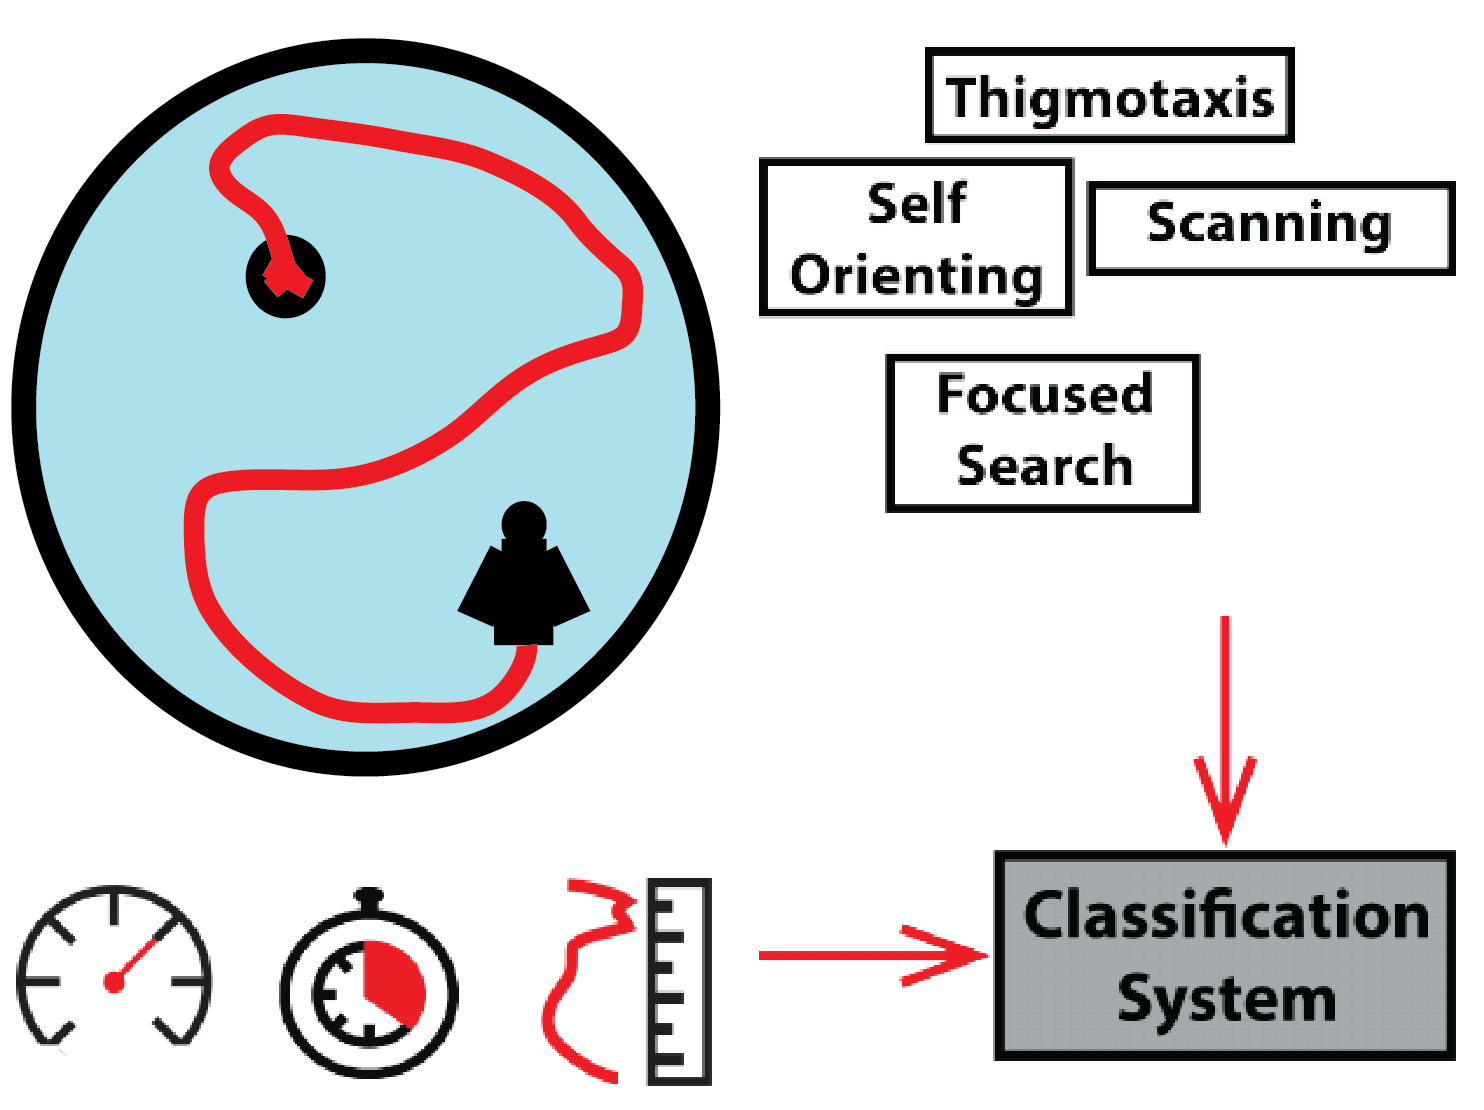
\includegraphics[width=0.8\textwidth]{figures/othersX1}}
		\onslide<2>\centerline{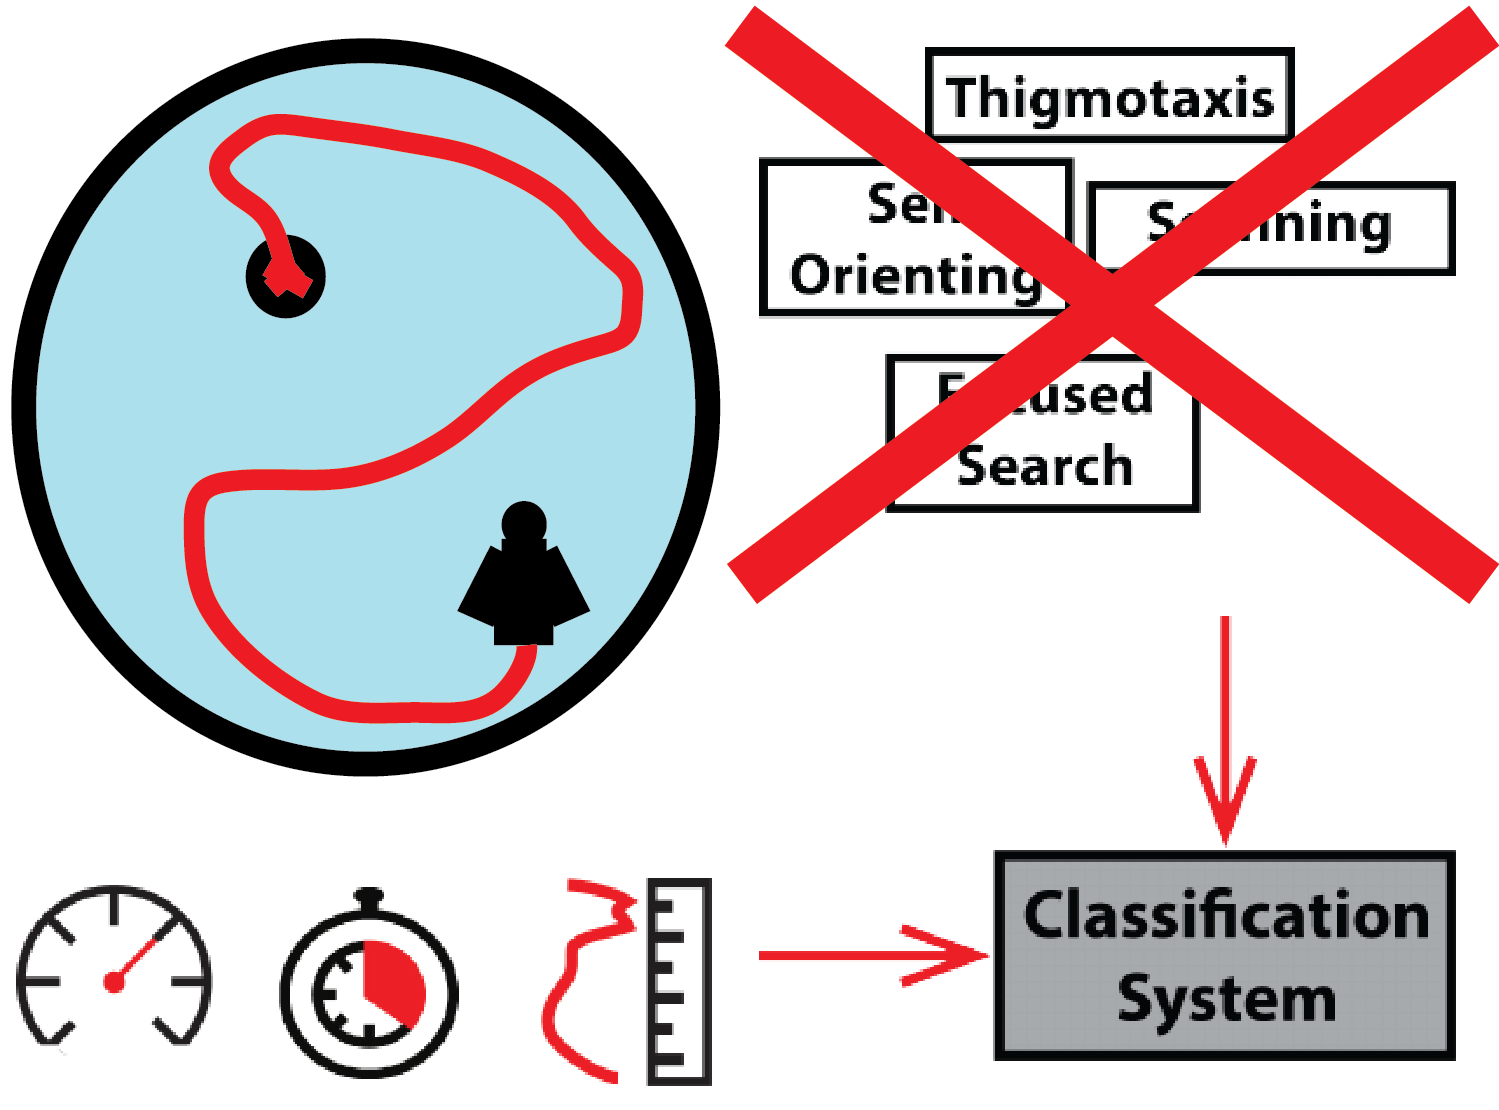
\includegraphics[width=0.8\textwidth]{figures/othersX2}}
		\onslide<3>\centerline{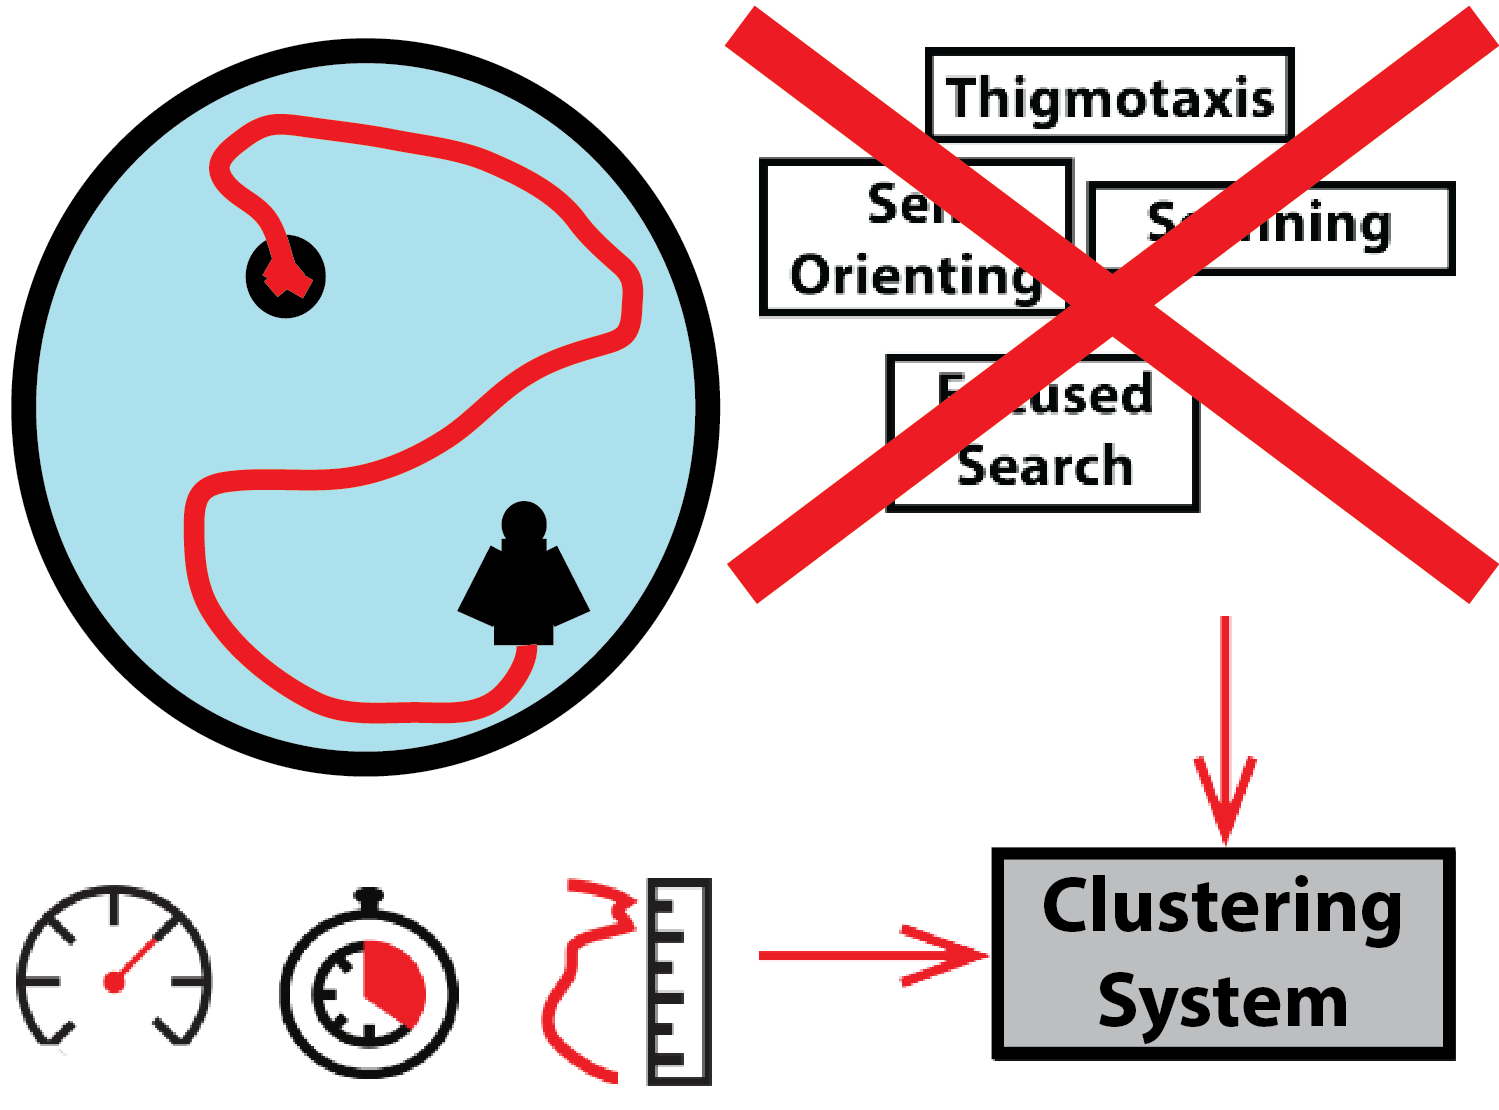
\includegraphics[width=0.8\textwidth]{figures/othersX3}}
	\end{overprint}
\end{figure}		
\end{frame}

\begin{frame}{Why don't we just apply the same frameworks?}
	\begin{figure}[H]
		\centering
		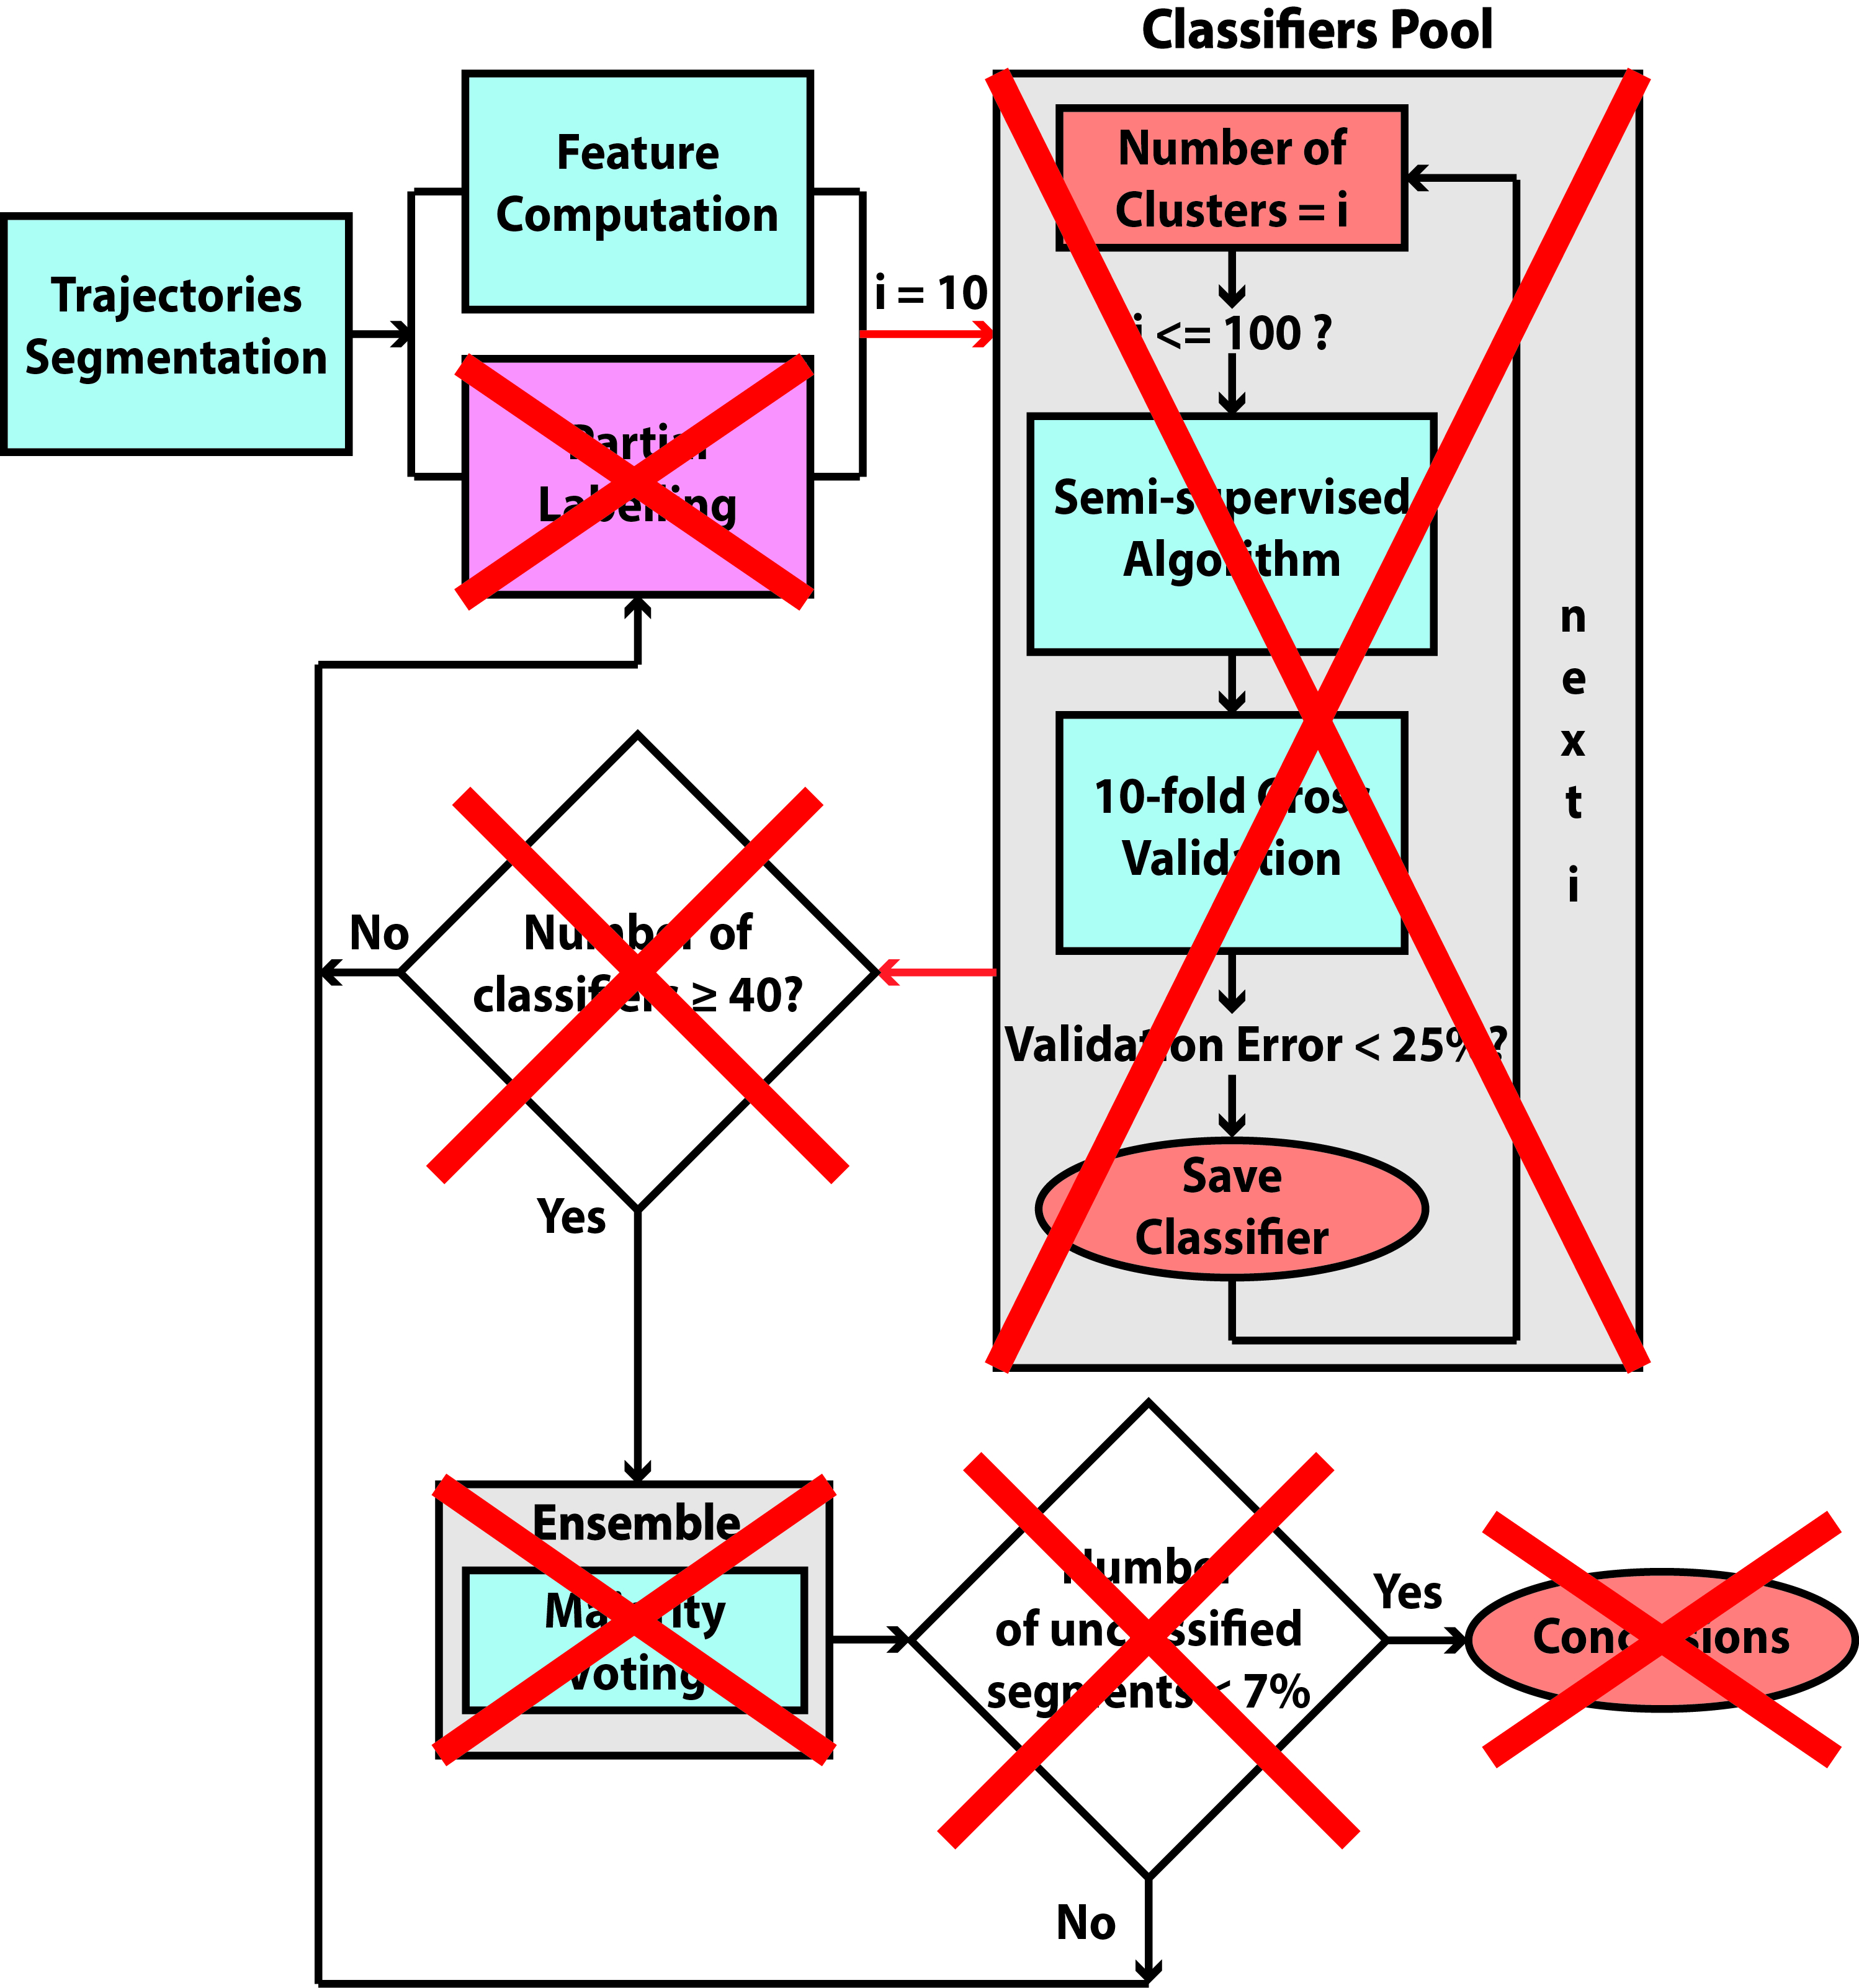
\includegraphics[width=0.6\textwidth]{figures/vourosetal2}
	\end{figure}	
\end{frame}

\begin{frame}{Let's just do clustering}
	\begin{figure}[H]
		\centering
		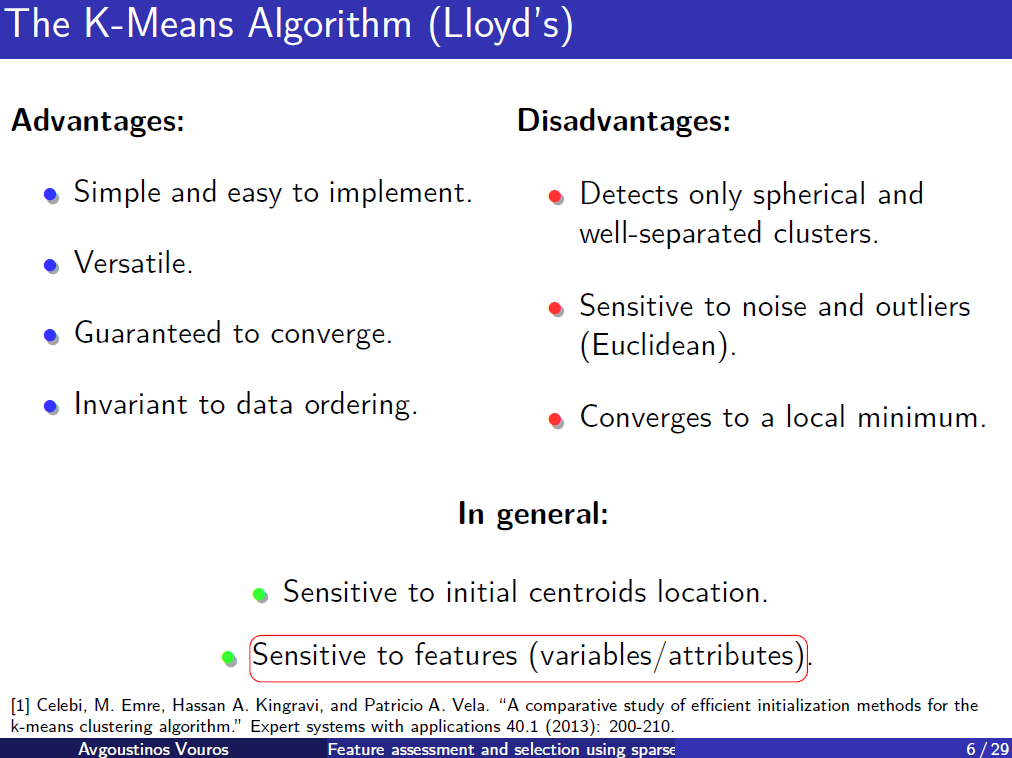
\includegraphics[width=0.9\textwidth]{figures/prev1}
	\end{figure}	
\end{frame}

\begin{frame}{Let's just do clustering}
\begin{itemize}
	\item<1->
	\begin{itemize}
		\item[{\MyShadow{$\bullet$}{blue!80}}] \textbf{ROBIN [1] or DK-Means++ [2]:} Make K-Means deterministic. 
		\item[{\MyShadow{$\bullet$}{blue!80}}] \textbf{Sparse K-Means [3]:} Auto-assess the feature quality and discard the ones that do not contribute to the overall clustering.		
		\item[{\MyShadow{$\bullet$}{red!80}}] \textbf{Auto-tunable:} Ability to find optimal parameters automatically.
		\item[{\MyShadow{$\bullet$}{green!80}}] \textbf{Ability to detect redundant features.}
	\end{itemize}	
	\item<2->
	\begin{figure}[H]
		\centering
		
\includegraphics[width=0.67\textwidth]{figures/NAG2}
	\end{figure}
	\item<1->
	\begin{tiny}
		\begin{noindlist}
			\item $[1]$ Al Hasan, Mohammad, et al. "Robust partitional clustering by outlier and density insensitive seeding." Pattern Recognition Letters 30.11 (2009): 994-1002.
			\item $[2]$ Nidheesh, N., KA Abdul Nazeer, and P. M. Ameer. "An enhanced deterministic K-Means clustering algorithm for cancer subtype prediction from gene expression data." Computers in biology and medicine 91 (2017): 213-221.
			\item $[3]$ Witten, Daniela M., and Robert Tibshirani. ``A framework for feature selection in clustering.'' Journal of the American Statistical Association 105.490 (2010): 713-726.						
		\end{noindlist}
	\end{tiny}		
\end{itemize}	
\end{frame}

\begin{frame}{Can you make sense of abstract path features?}
	\begin{figure}
		\begin{overprint}
			\onslide<1>\centerline{
\includegraphics[width=0.7\textwidth]{figures/countries}}
			\onslide<2>\centerline{
\includegraphics[width=0.7\textwidth]{figures/countries2}}
			\onslide<3>\centerline{
\includegraphics[width=0.7\textwidth]{figures/countries3}}			
		\end{overprint}
	\end{figure}		
\end{frame}

\begin{frame}[plain,c]
	\vspace{1mm}
	\begin{center}
		\begin{itemize}
			\item<1-> \textbf{Sodium nitroprusside ameliorates hyperglycemia-induced anatomical, neurovascular, and behavioural defects in zebrafish larvae}
			\item<1->
			\begin{figure}[H]
				\centering
				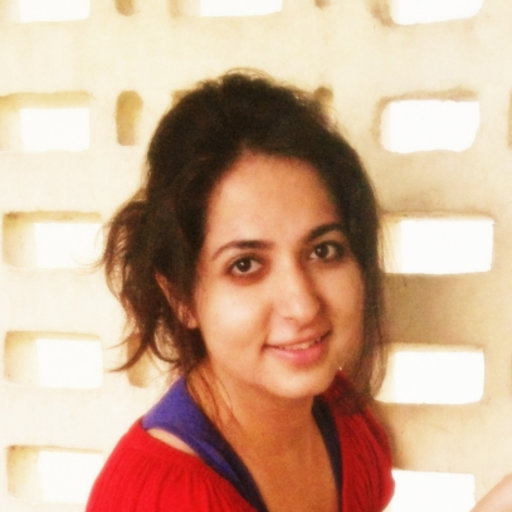
\includegraphics[width=0.4\textwidth]{figures/KC}
			\end{figure}
		\end{itemize}	
		\textit{\hphantom{xxxx} Dr Karishma Chhabria}
	\end{center}
\end{frame}

\begin{frame}{Sodium nitroprusside ameliorates hyperglycemia-induced anatomical, neurovascular, and behavioural defects in zebrafish larvae}
	\begin{itemize}[label={\MyShadow{$\bullet$}{blue!80}}]
		\item<1-> \textbf{Glucose:} provides energy by breaking down carbohydrates from food or drink.
		\item<2-> \textbf{Insulin:} (hormone) allows glucose to enter cells and fuel them with energy.		
		\item<3-> \textbf{Diabetes:} too much glucose in our blood because of reduced levels of insulin. Causes neurological disorders including cognitive impairment.
	\end{itemize}
	\begin{itemize}[label={\MyShadow{$\bullet$}{red!80}}]
		\item<4-> More specifically, diabetes impairs the neurovascular coupling (NVC) which is the connection between neurons and their energy source (vascular supply).
		\item<5-> Treatment with sodium nitroprusside (SNP) rescued this effect [1].
		\item<6-> The current work examines the effects of glucose exposure to the components of the neurovascular unit (NVU).
	\end{itemize}
	\begin{itemize}
	\item<5->\tiny{Chhabria, Karishma, et al. "The effect of hyperglycemia on neurovascular coupling and cerebrovascular patterning in zebrafish." Journal of Cerebral Blood Flow \& Metabolism (2018): 0271678X18810615.}	
	\end{itemize}
\end{frame}

\begin{frame}{\textbf{Behavioural analysis:} Sodium nitroprusside ameliorates hyperglycemia-induced anatomical, neurovascular, and behavioural defects in zebrafish larvae}
\begin{figure}
	\begin{overprint}
		\onslide<1>\centerline{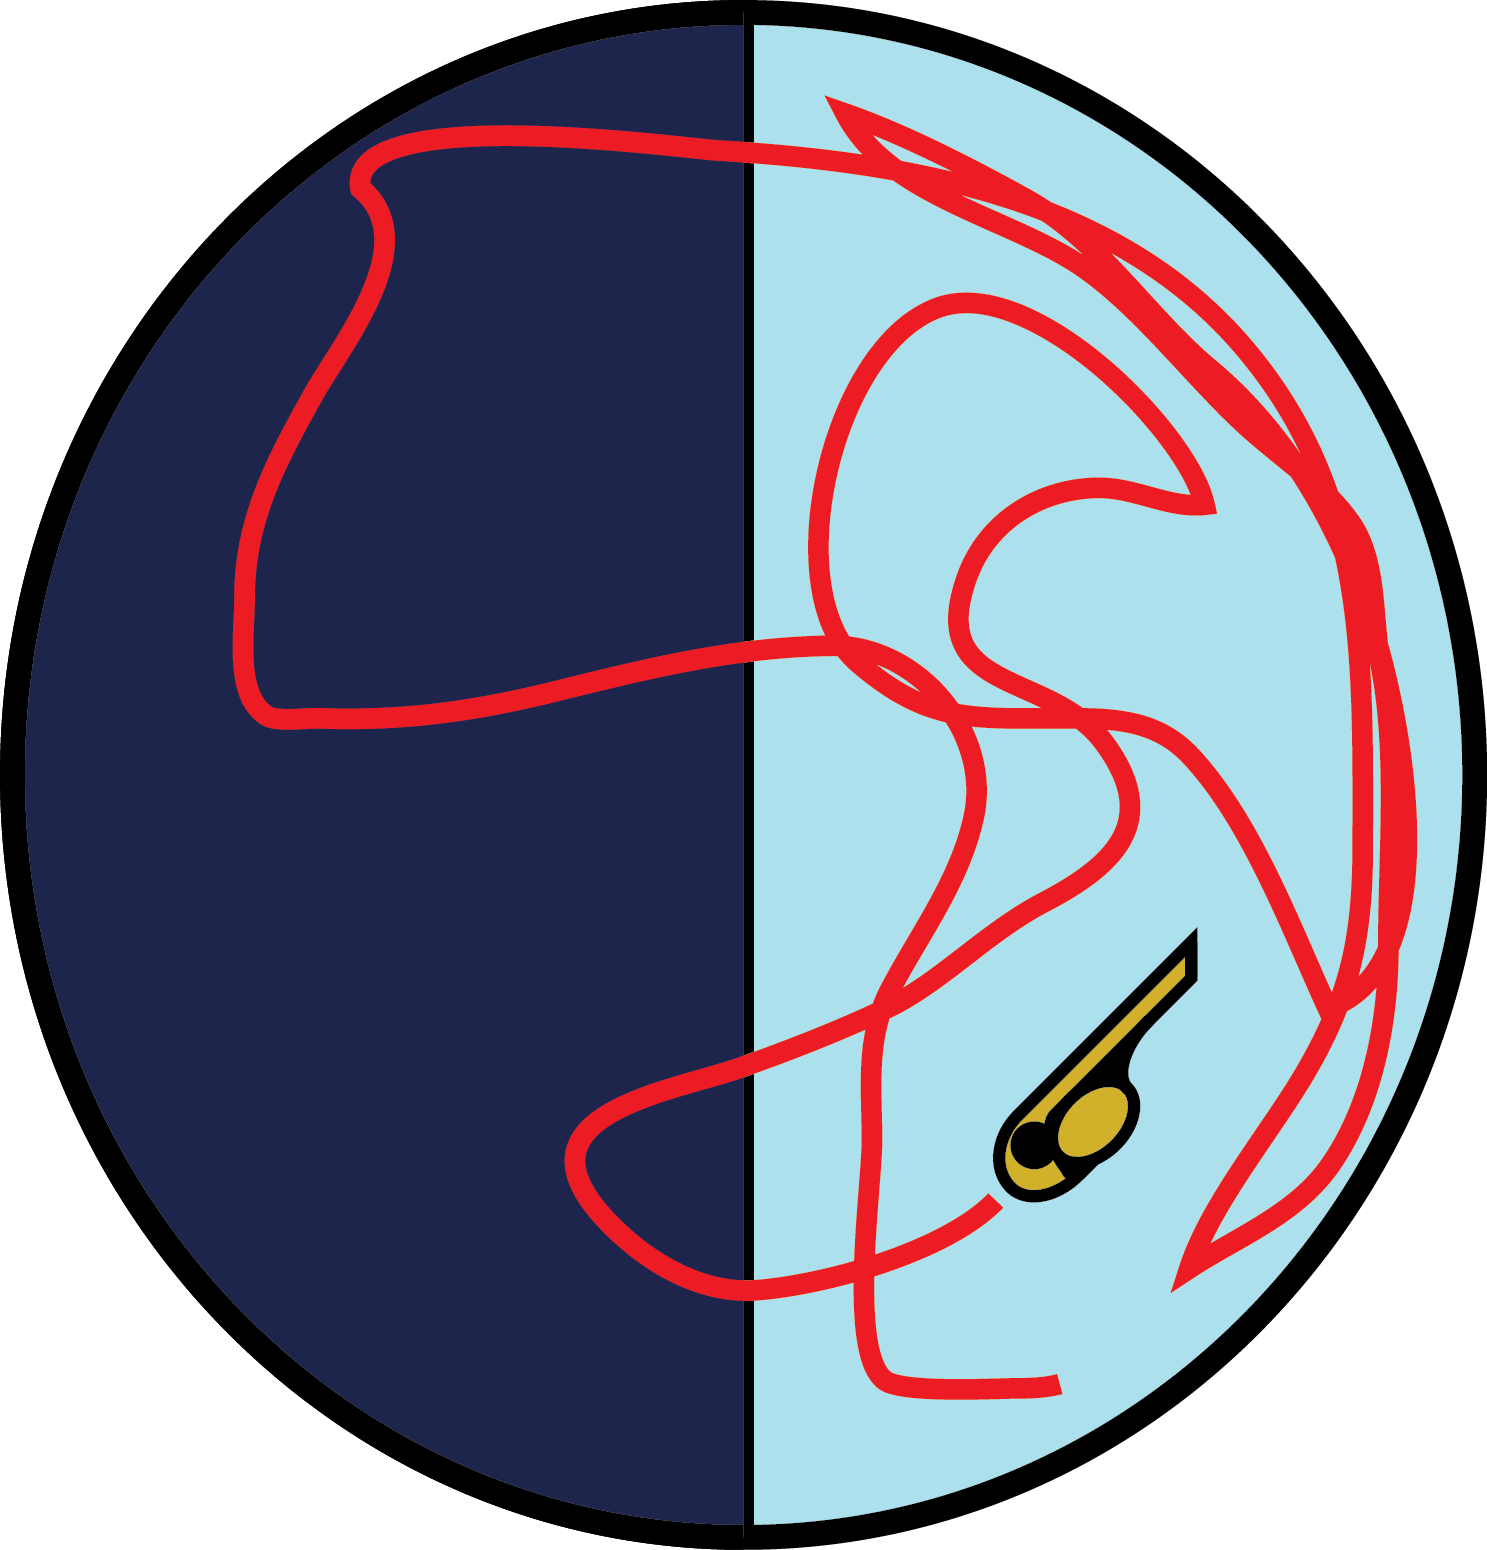
\includegraphics[width=0.4\textwidth]{figures/zebrafish}}
		\onslide<2>\centerline{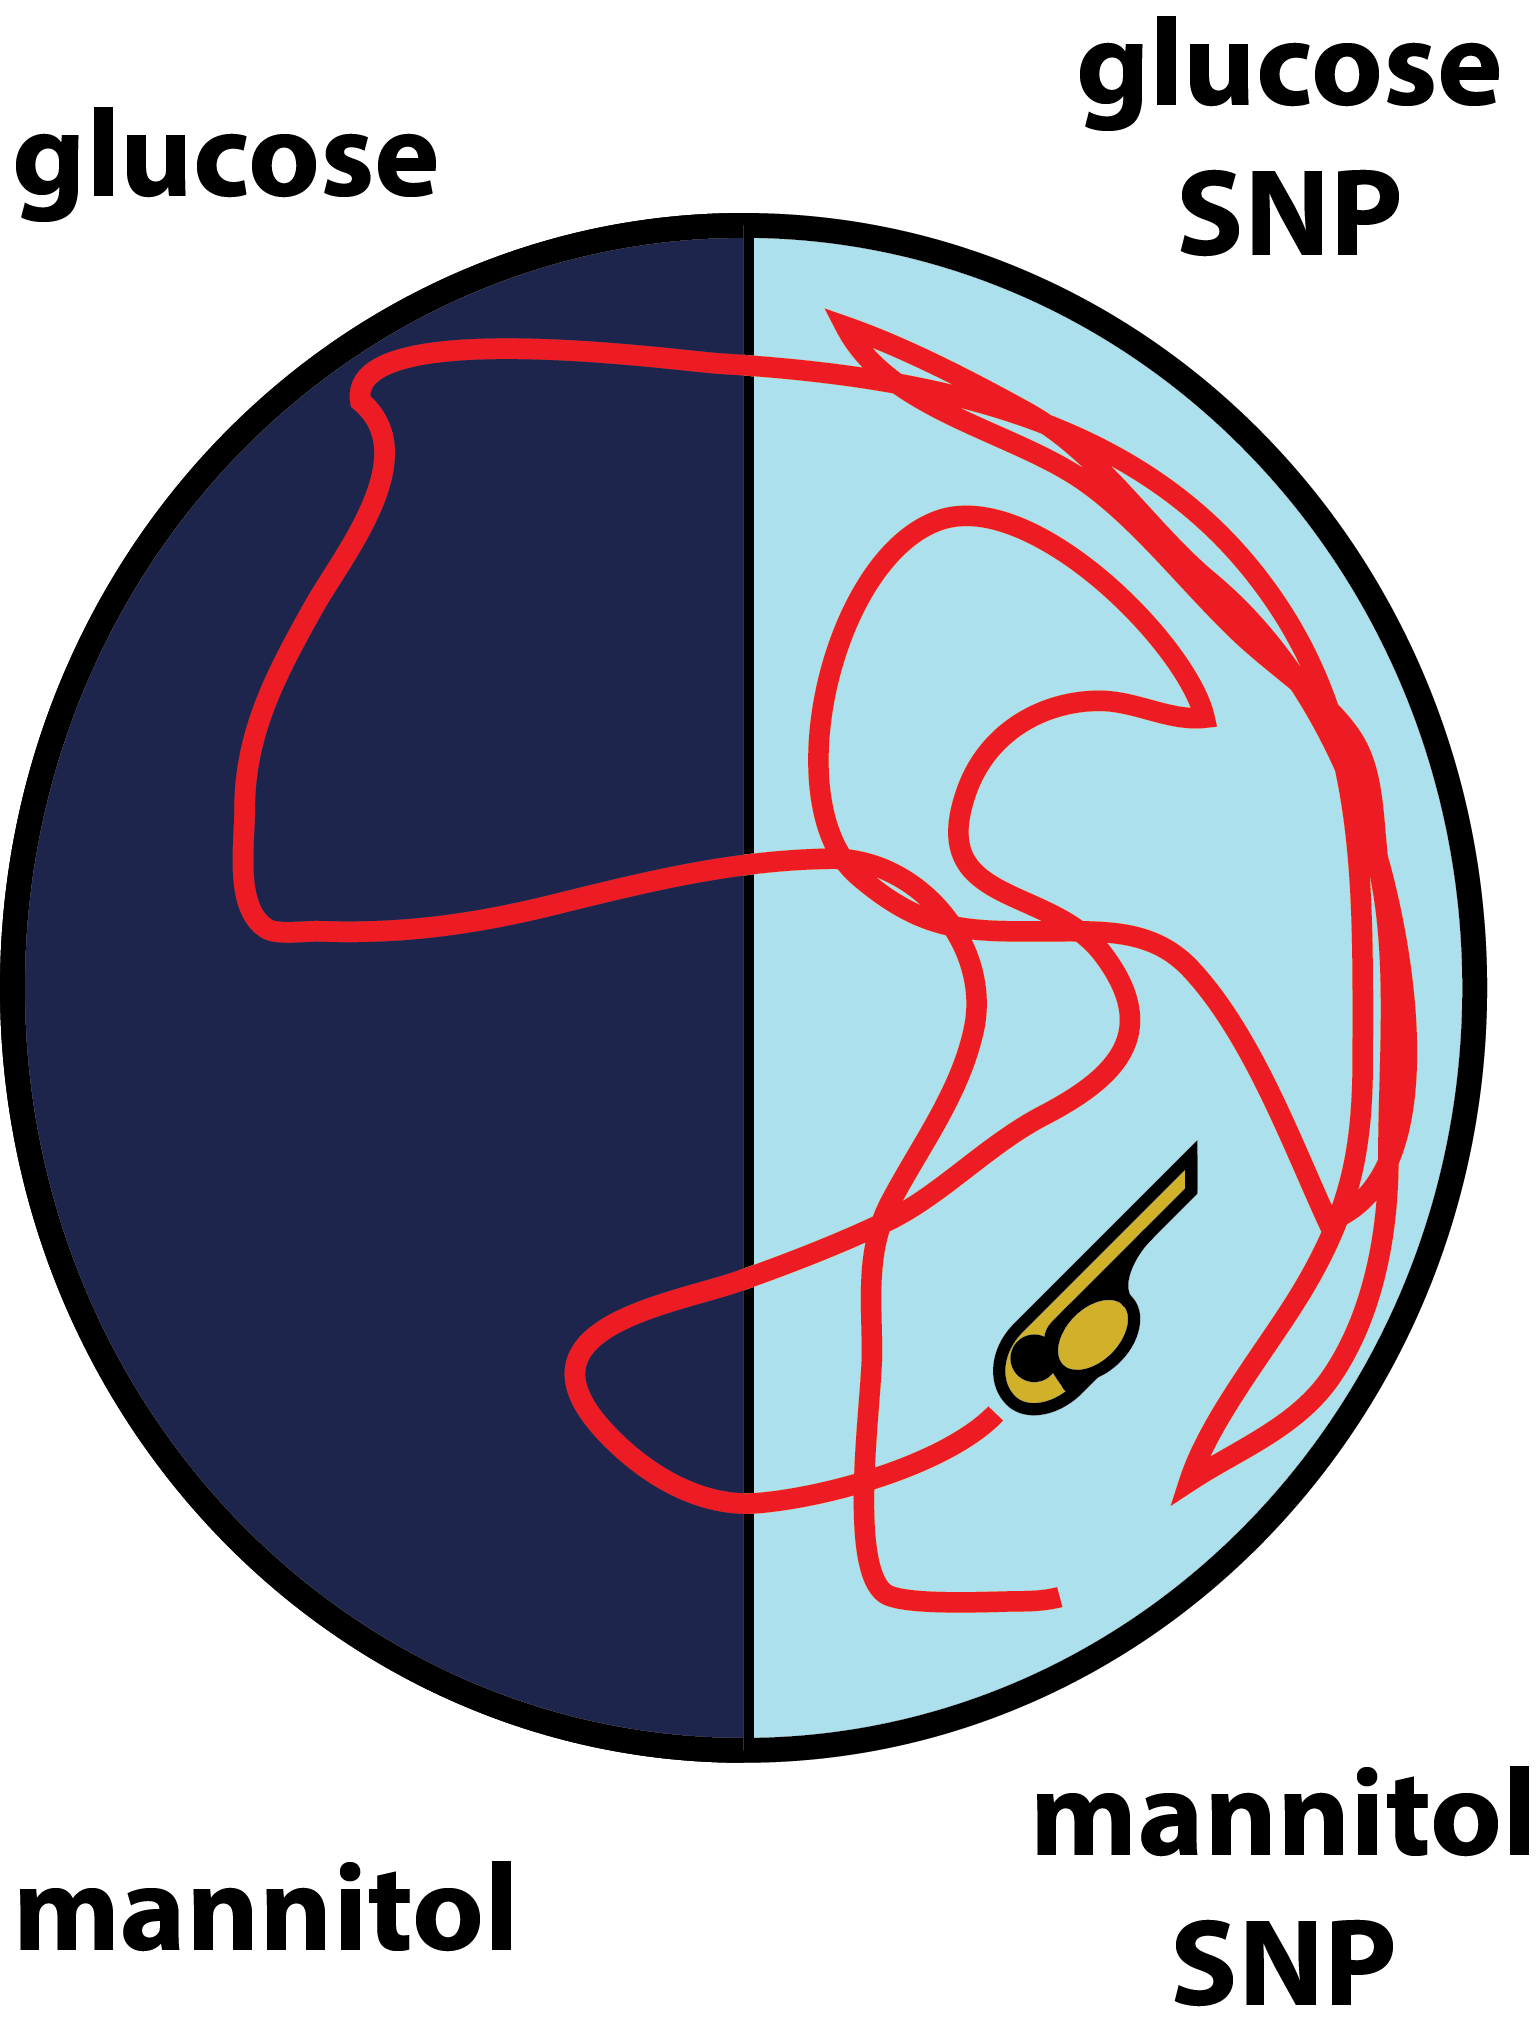
\includegraphics[width=0.4\textwidth]{figures/zebrafish2}}
	\end{overprint}
\end{figure}	
\end{frame}

\begin{frame}{\textbf{Behavioural analysis:} Segmentation}
\begin{figure}
	\begin{overprint}
		\onslide<1>\centerline{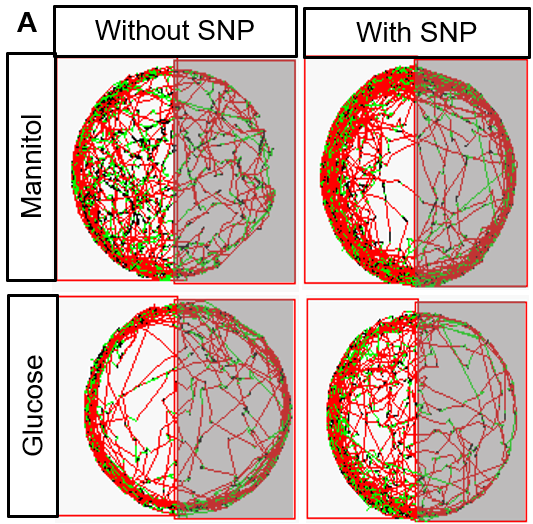
\includegraphics[width=0.6\textwidth]{figures/segmentation}}
		\onslide<2>\centerline{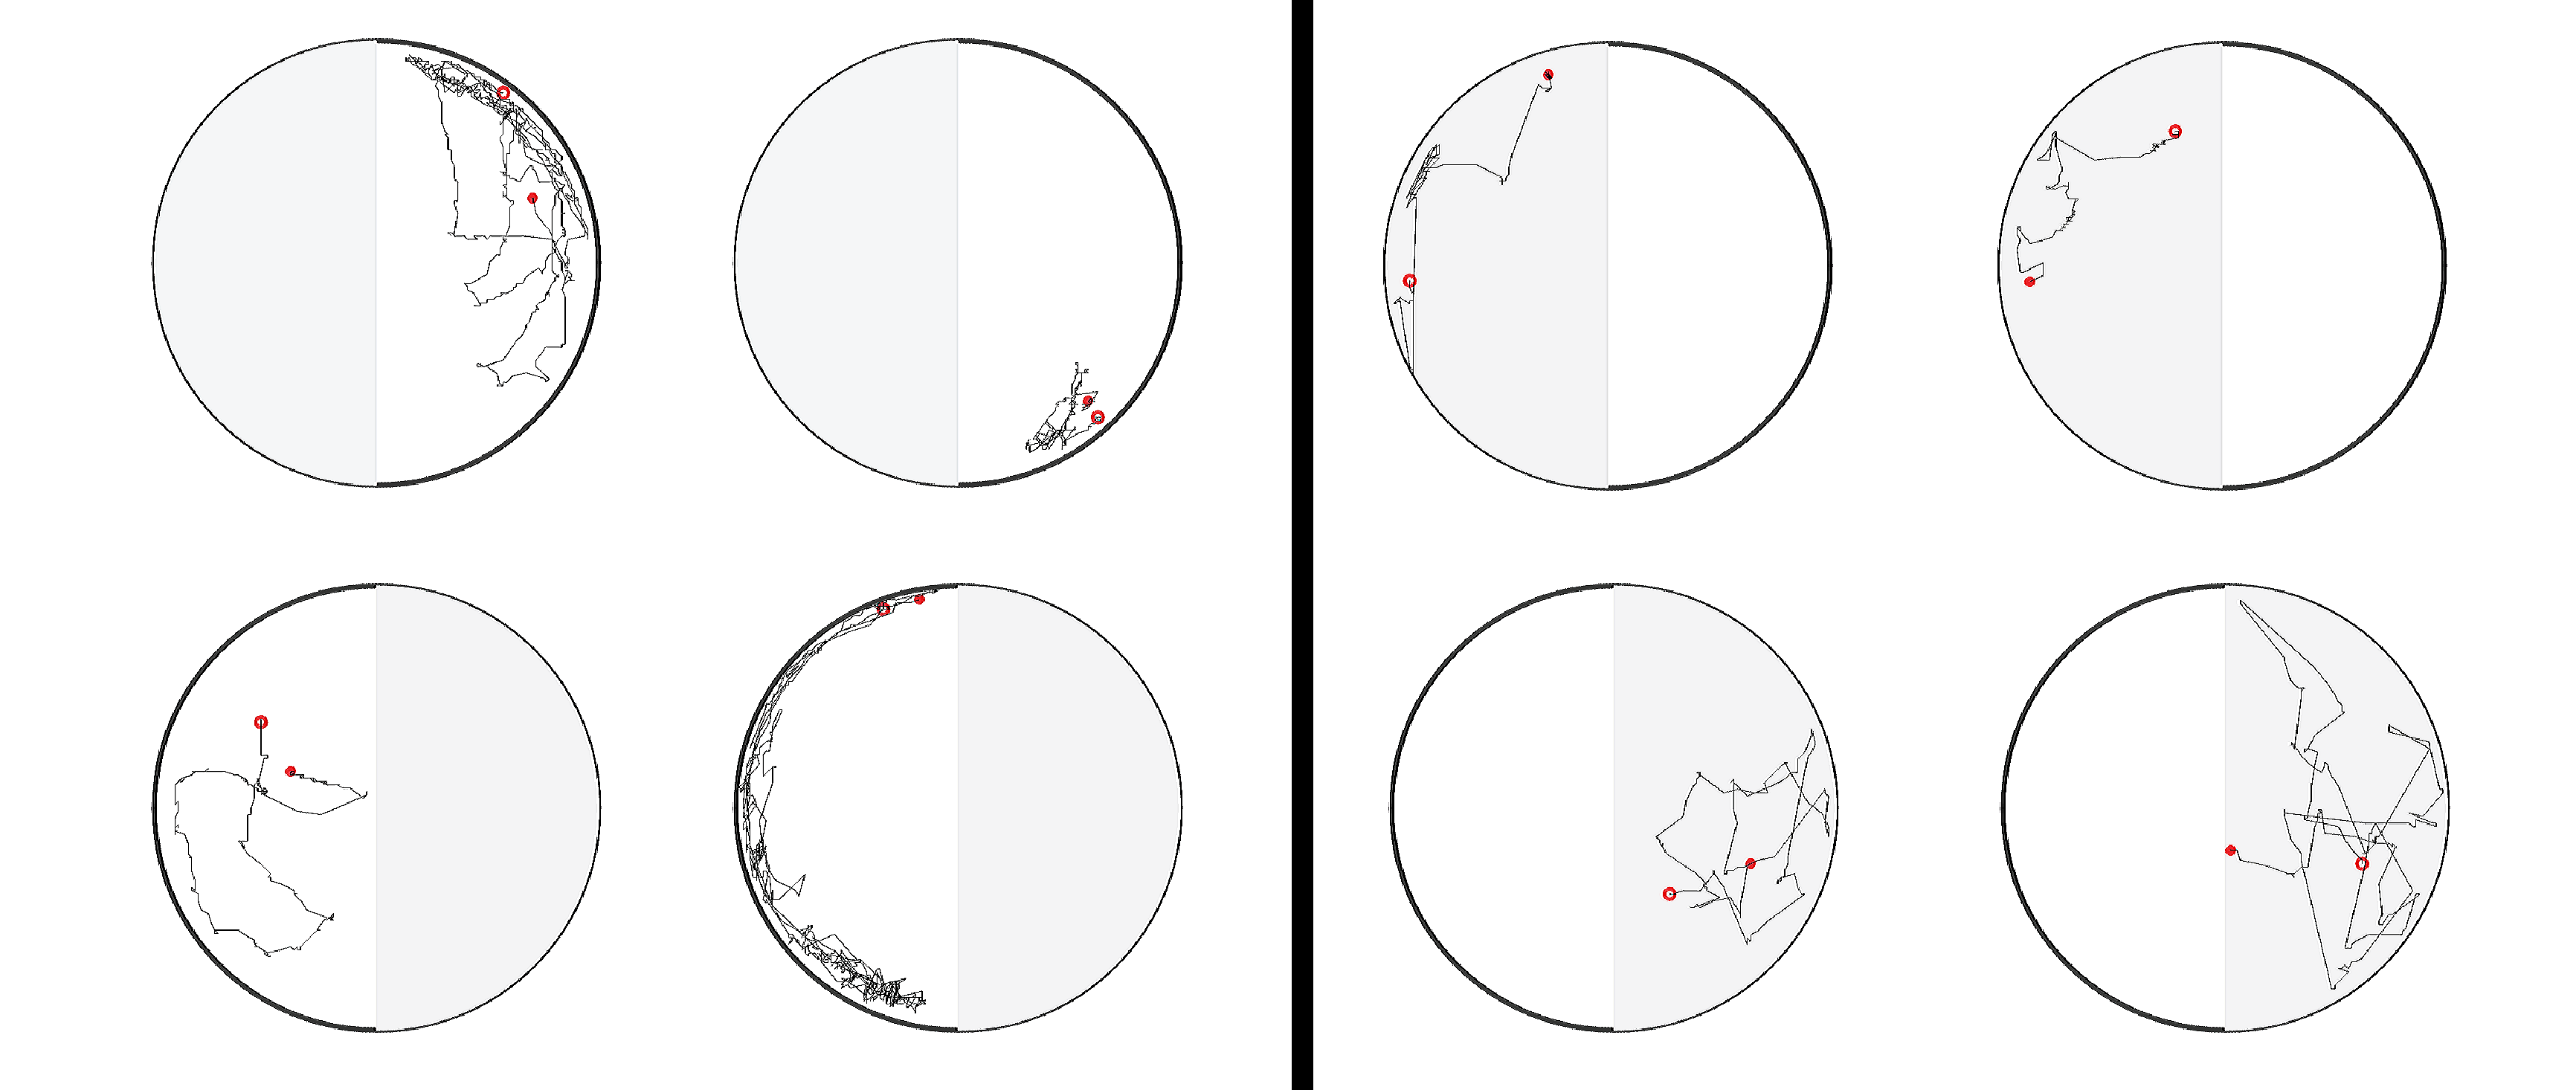
\includegraphics[width=\textwidth]{figures/segmentation2}}
	\end{overprint}
\end{figure}	
\end{frame}

\begin{frame}{\textbf{Behavioural analysis:} Path features}
	\begin{figure}[H]
		\centering
		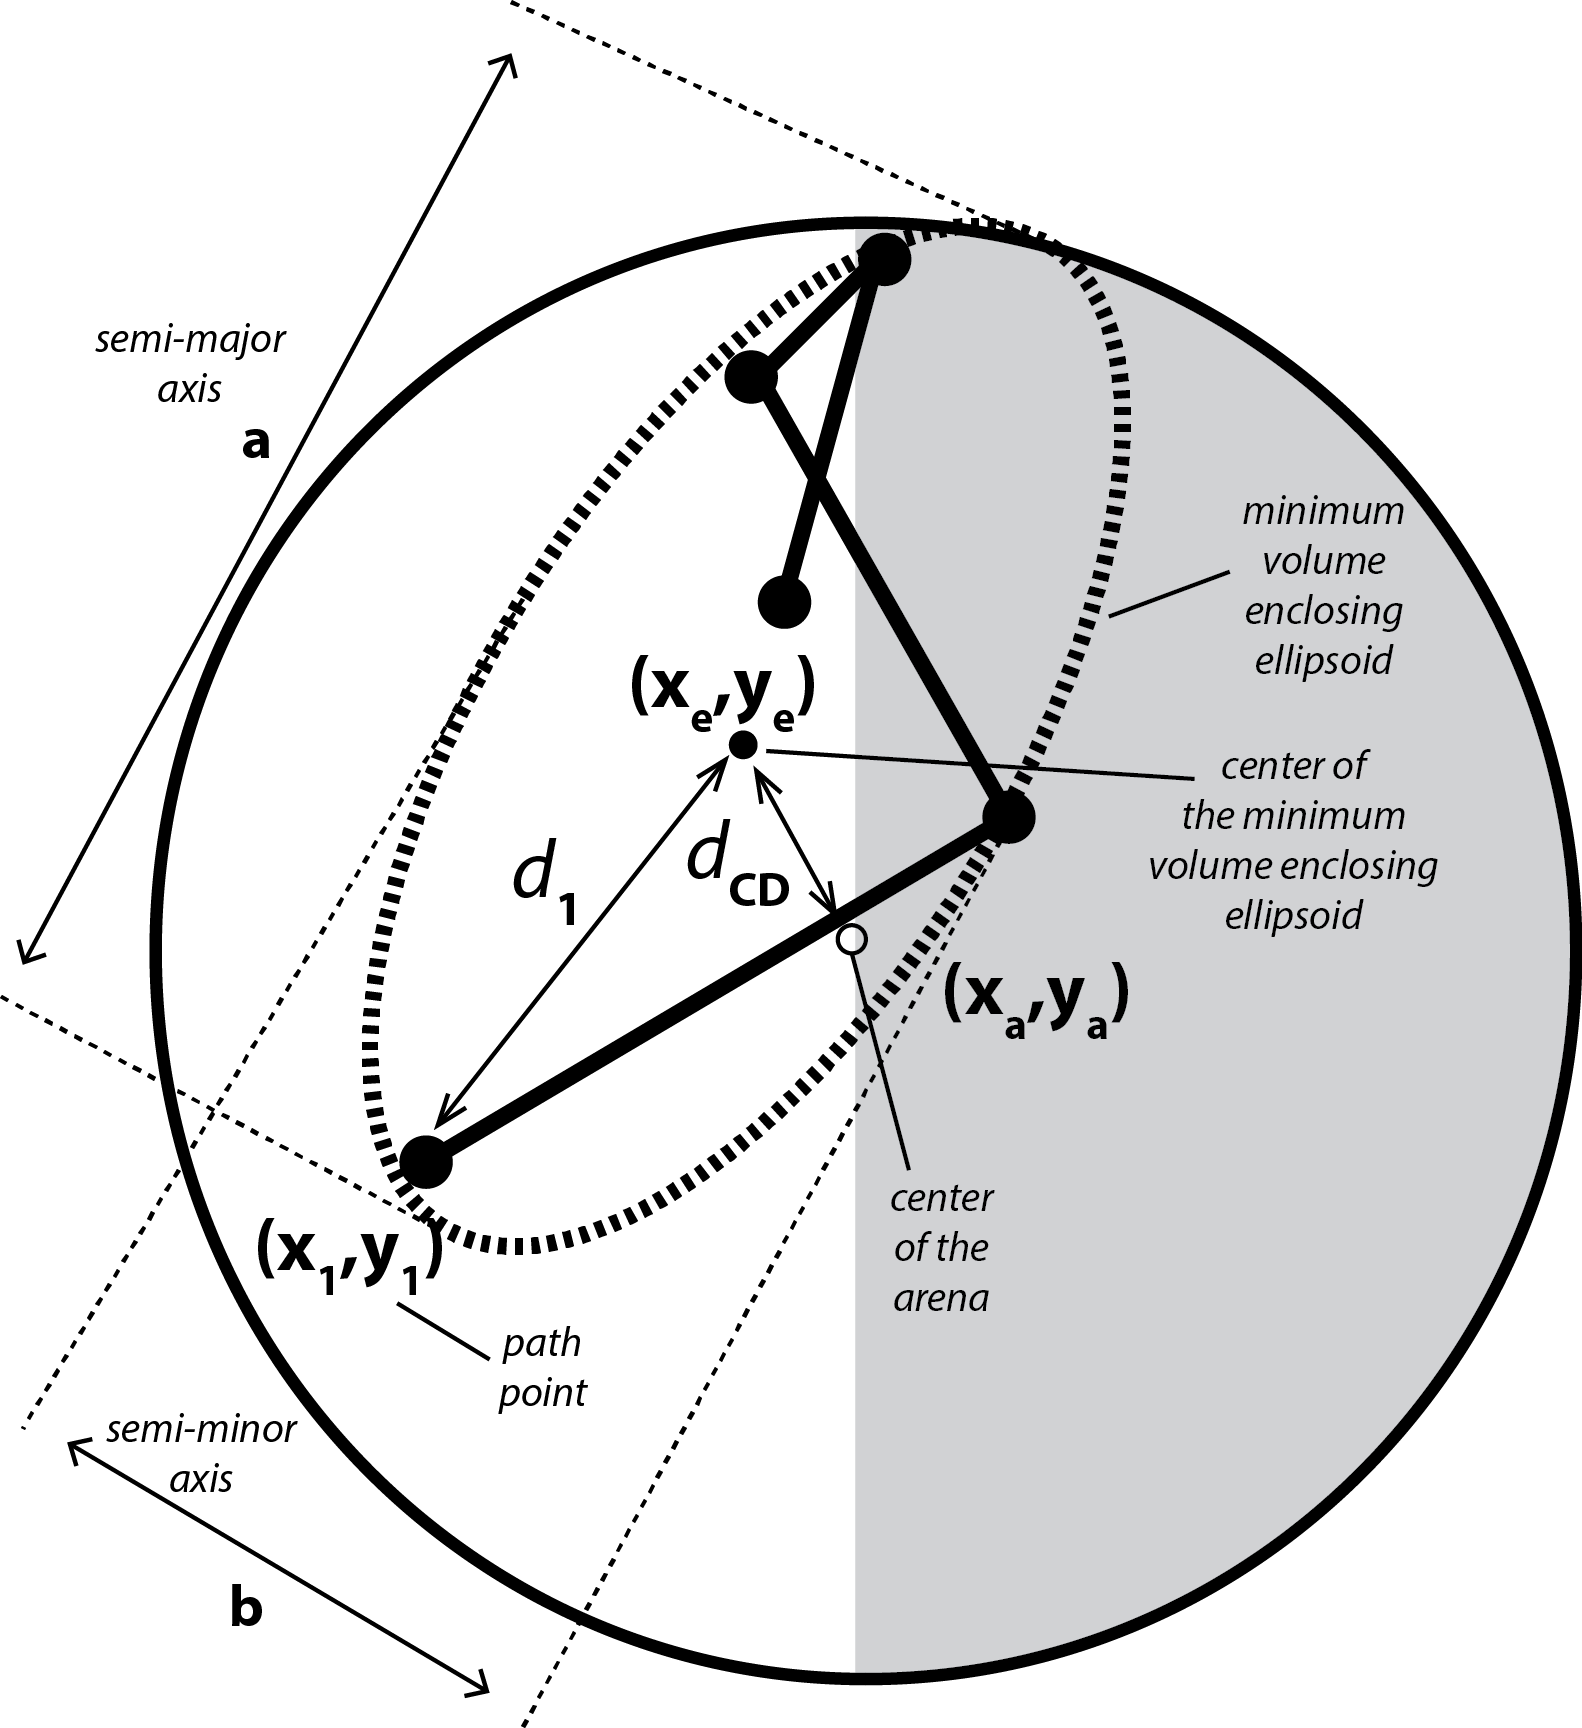
\includegraphics[width=0.6\textwidth]{figures/zebrafishfeats}
	\end{figure}	
\end{frame}

\begin{frame}{\textbf{Behavioural analysis:} Path features}
	\begin{itemize}[label={\MyShadow{$\bullet$}{blue!80}}]
		\setlength\itemsep{2em}
		\item \textbf{Eccentricity [1]:} $\epsilon = \sqrt{(1-\frac{b^2}{a^2})}$
		\item \textbf{Mean path point distance from ellipsoid:} $MPP = \frac{\sum_{i=1}^{n}\sqrt{(x_i-x_e)^2 + (y_i-y_e)^2}}{n}$
		\item \textbf{Central displacement [1]:} $d_{CD} = \sqrt{(x_e-x_a)^2 + (y_e-y_a)^2}$ 
		\item \textbf{Number of entrances/exits:} number of transitions between light and dark side of the arena.
	\end{itemize}	
	\vspace{10mm}
	\tiny{Gehring, Tiago V., et al. "Detailed classification of swimming paths in the Morris Water Maze: multiple strategies within one trial." Scientific reports 5 (2015): 14562.}
\end{frame}

\begin{frame}{\textbf{Behavioural analysis:} Path features}
	\begin{figure}[H]
		\centering
		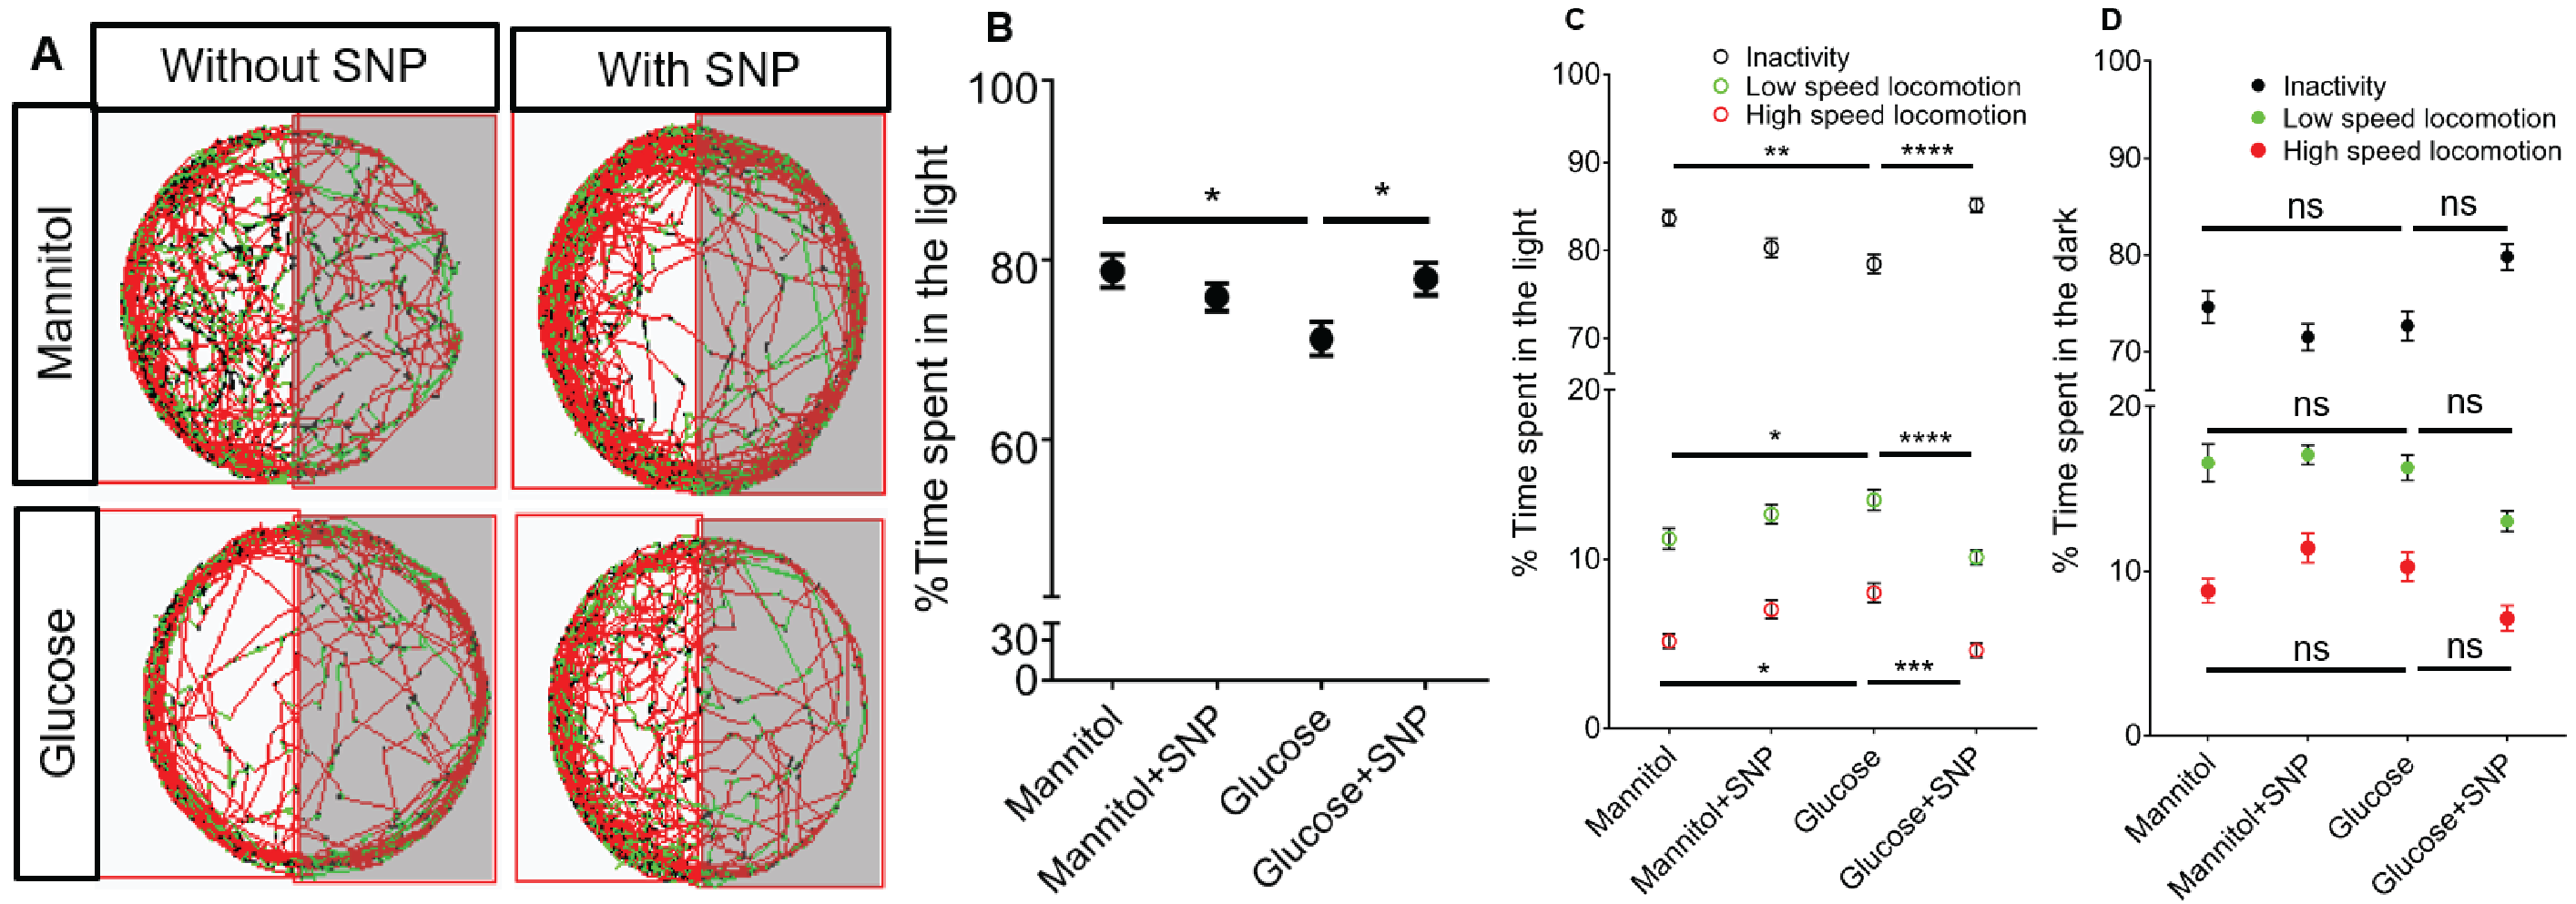
\includegraphics[width=\textwidth]{figures/results1}
	\end{figure}	
\end{frame}

\begin{frame}{\textbf{Behavioural analysis:} Path features}
	\begin{figure}[H]
		\centering
		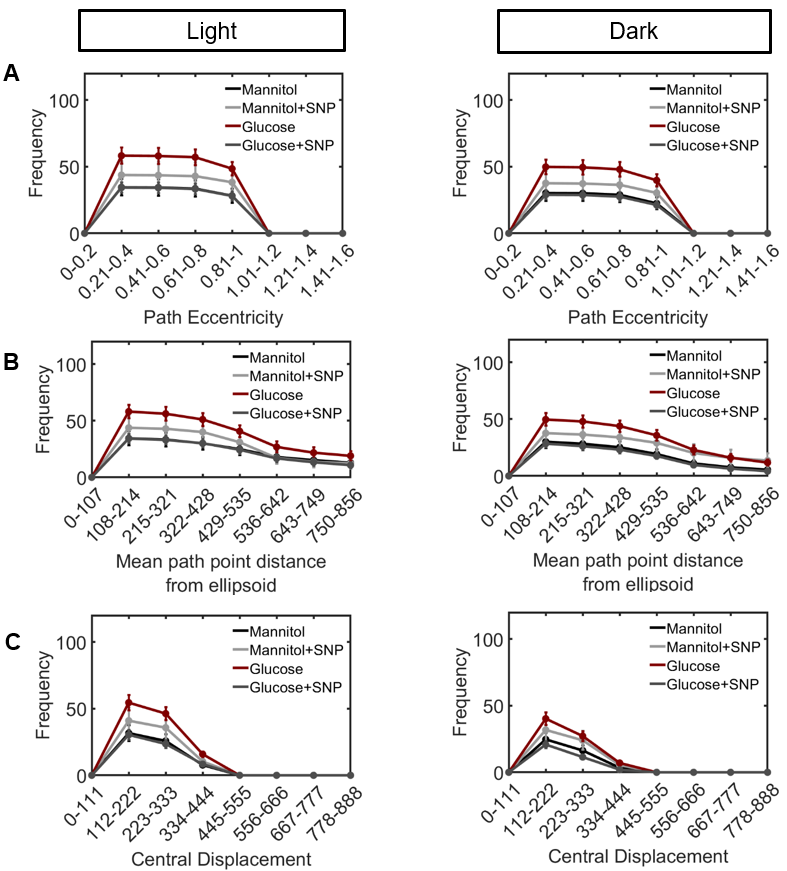
\includegraphics[width=0.6\textwidth]{figures/results2}
	\end{figure}	
\end{frame}

\begin{frame}{\textbf{Behavioural analysis}}
	\begin{figure}[H]
		\centering
		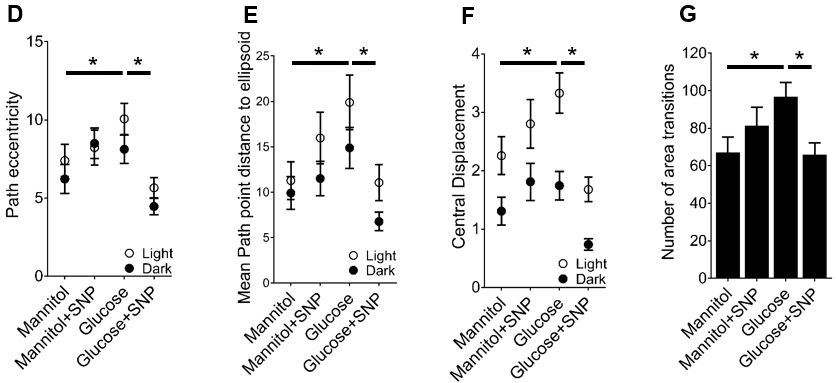
\includegraphics[width=\textwidth]{figures/results3}
	\end{figure}	
\end{frame}

\begin{frame}{\textbf{Behavioural analysis:} Results}
	\begin{itemize}
		\item<1->{\MyShadow{$\bullet$}{red!80}} Glucose exposure reduced light-dark preference which was rescued by co-treatment with SNP.
		\item<2->{\MyShadow{$\bullet$}{red!80}} Glucose exposure resulted in a significant increase in the time larvae spent undertaking both low and high speed locomotion while in the light region of the well, with an associated reduction in the time spent inactive. SNP co-treatment reversed this effect.
		\item<3->{\MyShadow{$\bullet$}{blue!80}} Quantifying the same measures for the dark region of the well, we found similar trends to that seen in light area but these were non-significant.
	\end{itemize}
\end{frame}

\begin{frame}{\textbf{Behavioural analysis:} Results}
	\begin{itemize}
		\item<1->{\MyShadow{$\bullet$}{red!80}} Glucose exposed larvae showed an increase in path eccentricities, mean PPDE and central displacement compared to mannitol exposed larvae and co-treatment with SNP rescued all these features in the light side of the well.
		\item<2->{\MyShadow{$\bullet$}{blue!80}} We did not observe significant differences in these features between glucose and mannitol with or without SNP in the dark side of the well. 
		\item<3->{\MyShadow{$\bullet$}{red!80}} We found that glucose exposure increased the number of transitions between these areas compared to mannitol treated larvae and this was rescued by co-treatment with SNP.
	\end{itemize}
\end{frame}

\begin{frame}{\textbf{Behavioural analysis:} Discussion}
	\begin{itemize}
		\item<1->{\MyShadow{$\bullet$}{red!80}} This is the first study characterizing the effect of hyperglycemia on geometrical and positional characteristics of zebrafish locomotion.
		\item<2->{\MyShadow{$\bullet$}{red!80}} Increase in positional and geometric features with glucose exposure implies an altered behaviour such as increased exploration and thigmotaxis.
		\item<3->{\MyShadow{$\bullet$}{blue!80}} Various zebrafish studies have shown increased exploration and thigmotaxis with anxiogenic drug treatments (Egan, Bergner et al. 2009, Blaser, Chadwick et al. 2010).  This further points to the associated of glucose exposure and diabetes to anxiety related brain activation and needs further investigation.
	\end{itemize}
\end{frame}

\begin{frame}[plain,c]
	%\frametitle{A first slide}
	\vspace{1mm}
	\begin{center}
		\Huge Future work on features
	\end{center}
\end{frame}

\begin{frame}{\textbf{Future work}}
	\begin{figure}[H]
		\centering
		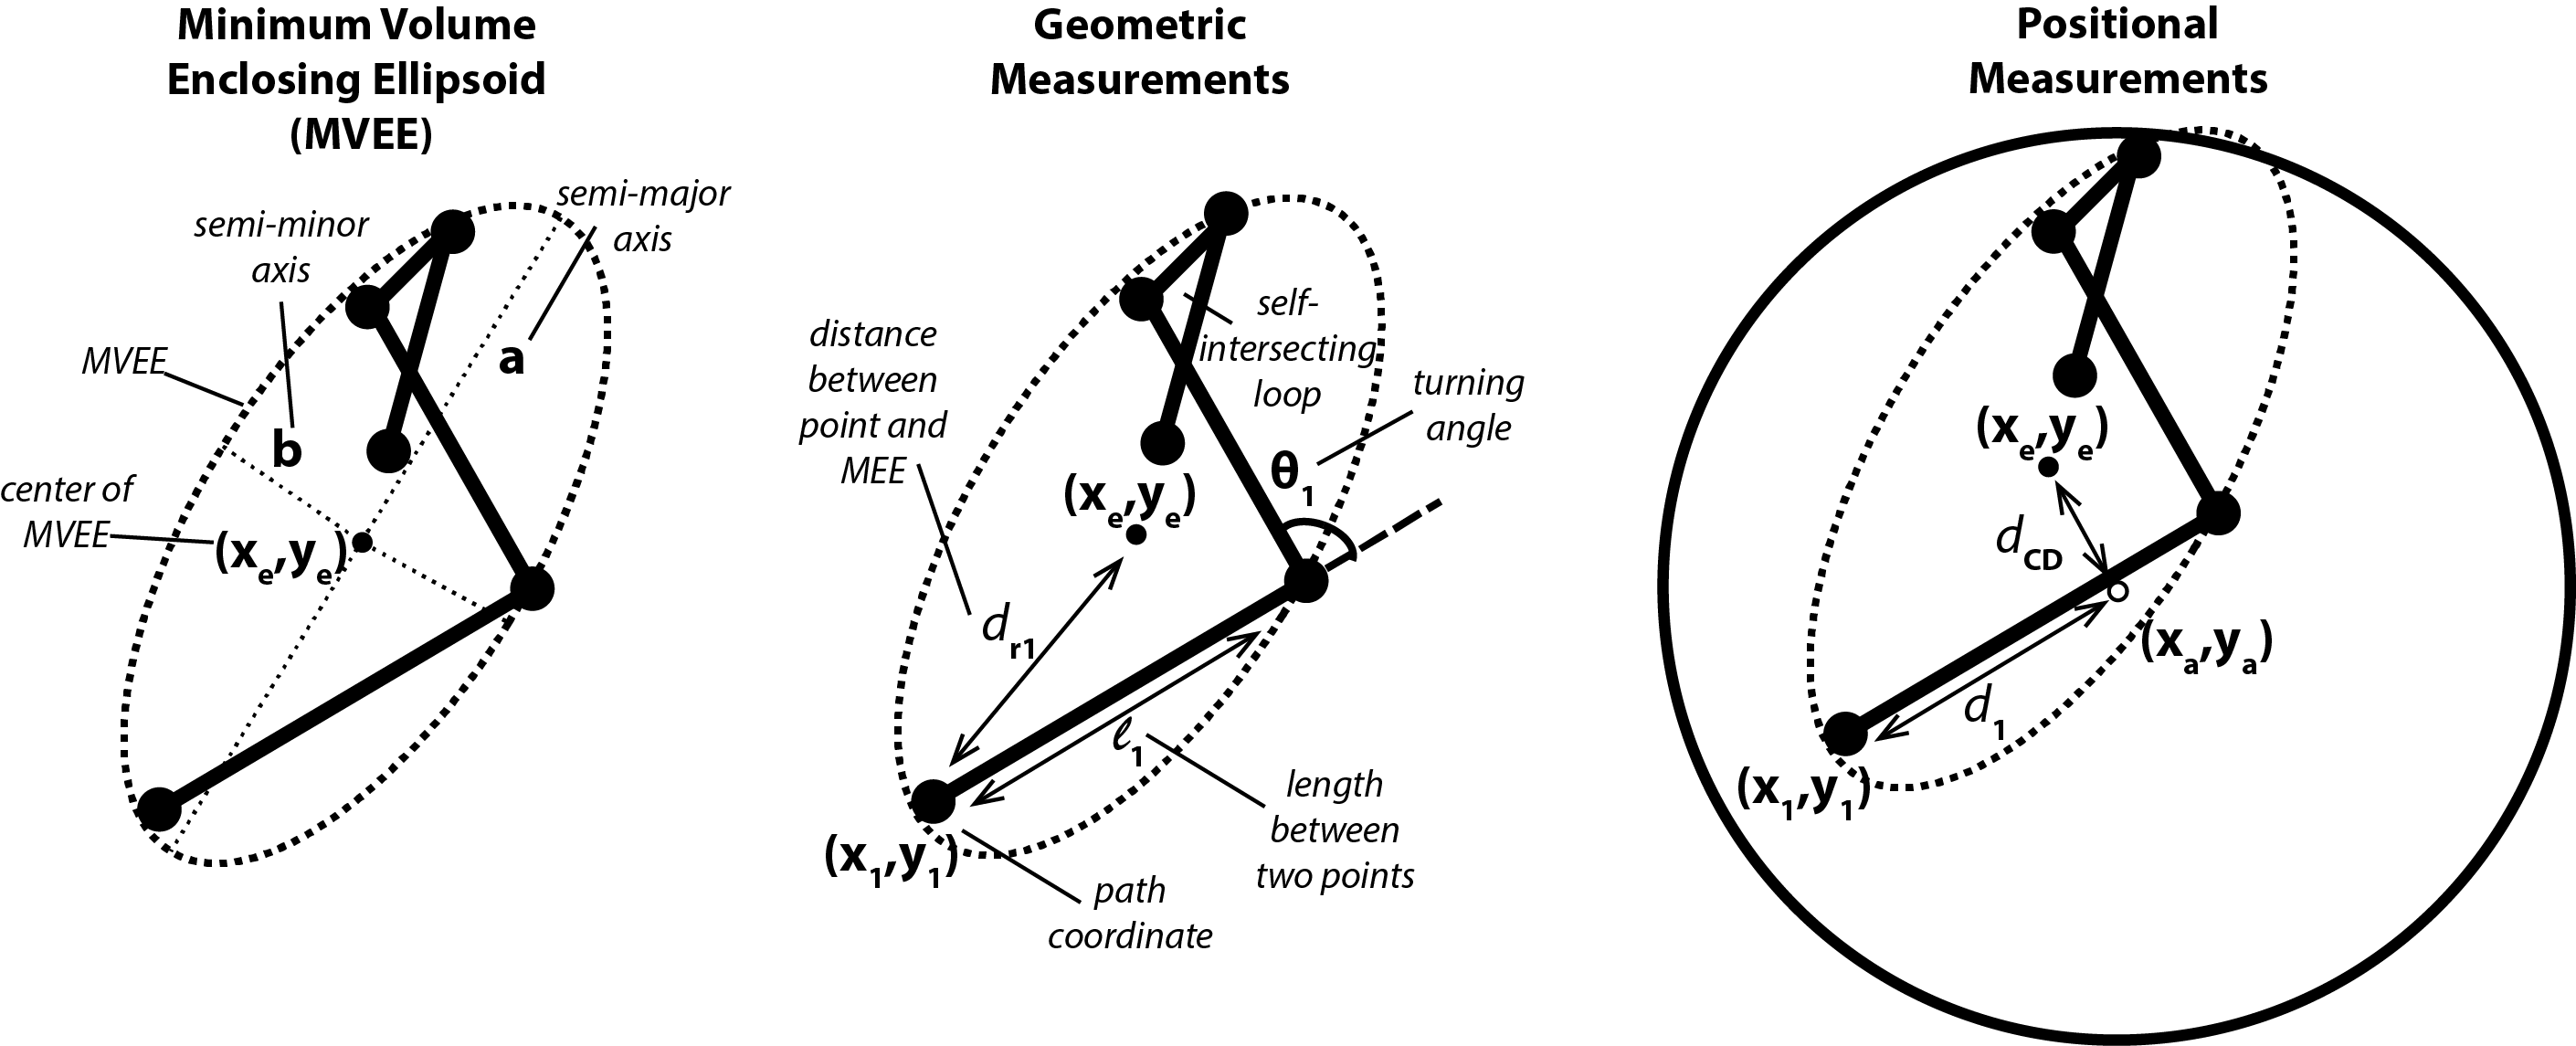
\includegraphics[width=\textwidth]{figures/pathfeatures1}
	\end{figure}	
\end{frame}

\begin{frame}{\textbf{Future work}}
	\begin{figure}[H]
		\centering
		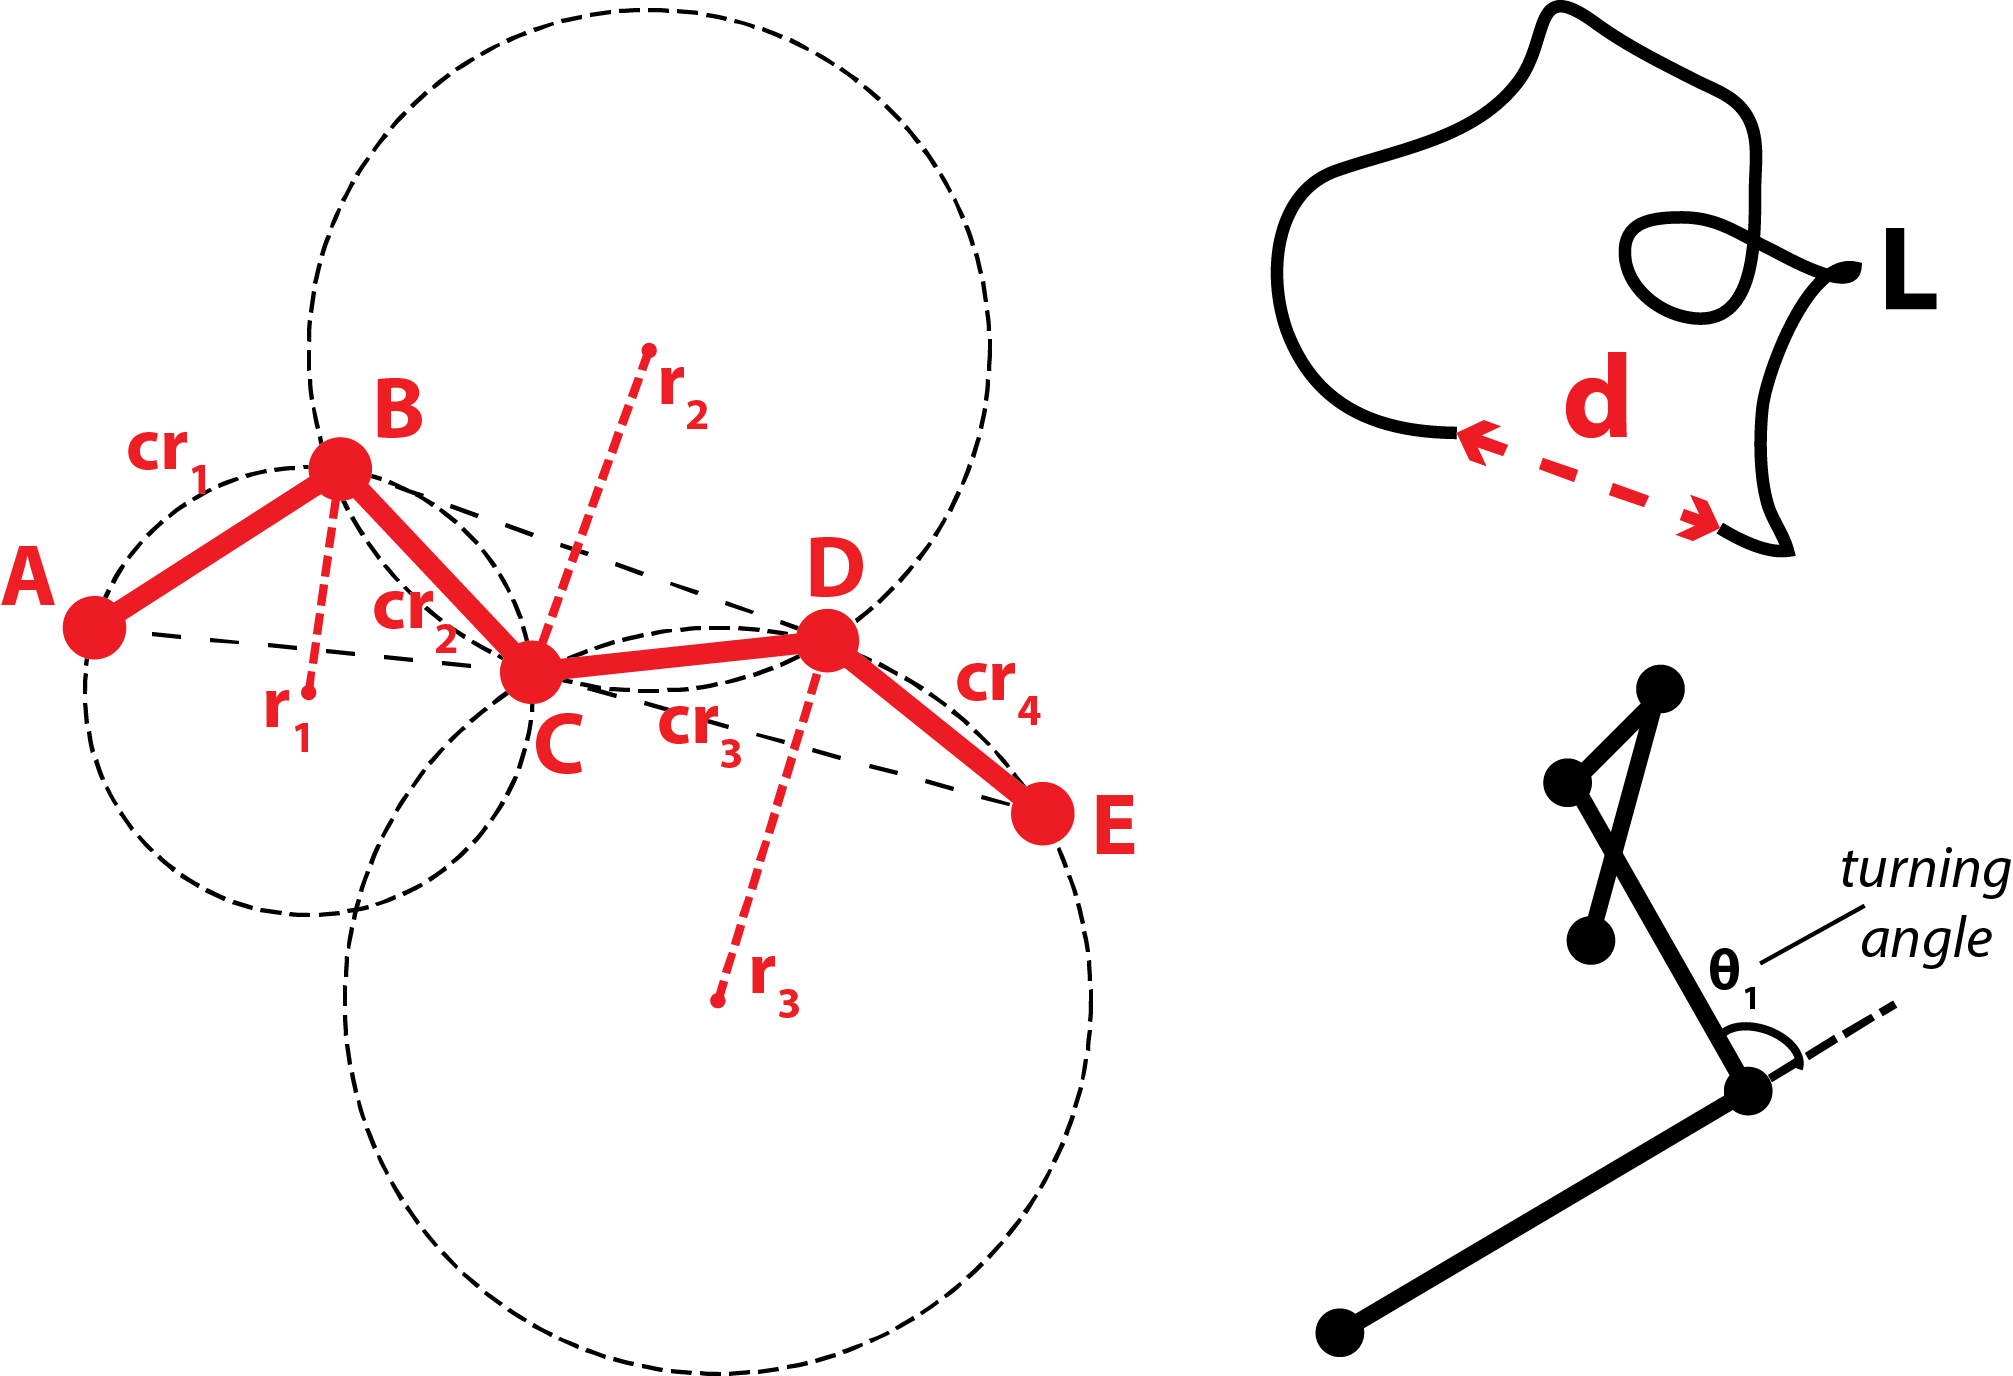
\includegraphics[width=0.9\textwidth]{figures/pathfeatures3}
	\end{figure}	
\end{frame}

\begin{frame}{\textbf{Future work}}
	\begin{equation}
		S1 = \frac{d}{L}
	\end{equation}
	\vspace{4mm}
	\begin{equation}
		S2 = 2\sqrt{p_m\frac{1+c}{1-c}+p_{cv}^2}
	\end{equation}	
	\vspace{4mm}
	\begin{equation}
		S3 = 2\sqrt{p_m\frac{1+c^2-s^2}{(1-c)^2+s^2}+p_{cv}^2}
	\end{equation}	
	\vspace{10mm}
	\tiny{
	\begin{itemize}
		\item $[1]$ Benhamou, Simon. "How to reliably estimate the tortuosity of an animal's path:: straightness, sinuosity, or fractal dimension?." Journal of theoretical biology 229.2 (2004): 209-220.
		\item $[2]$ Almeida, Paulo JAL, et al. "Indices of movement behaviour: conceptual background, effects of scale and location errors." Zoologia 27.5 (2010).
	\end{itemize}
	}		
\end{frame}

\begin{frame}[plain,c]
	\begin{Large}
		\begin{center}
			\textbf{Thank you for your attention!}
		\end{center}
	\end{Large}	
	\begin{figure}[H]
		\centering
		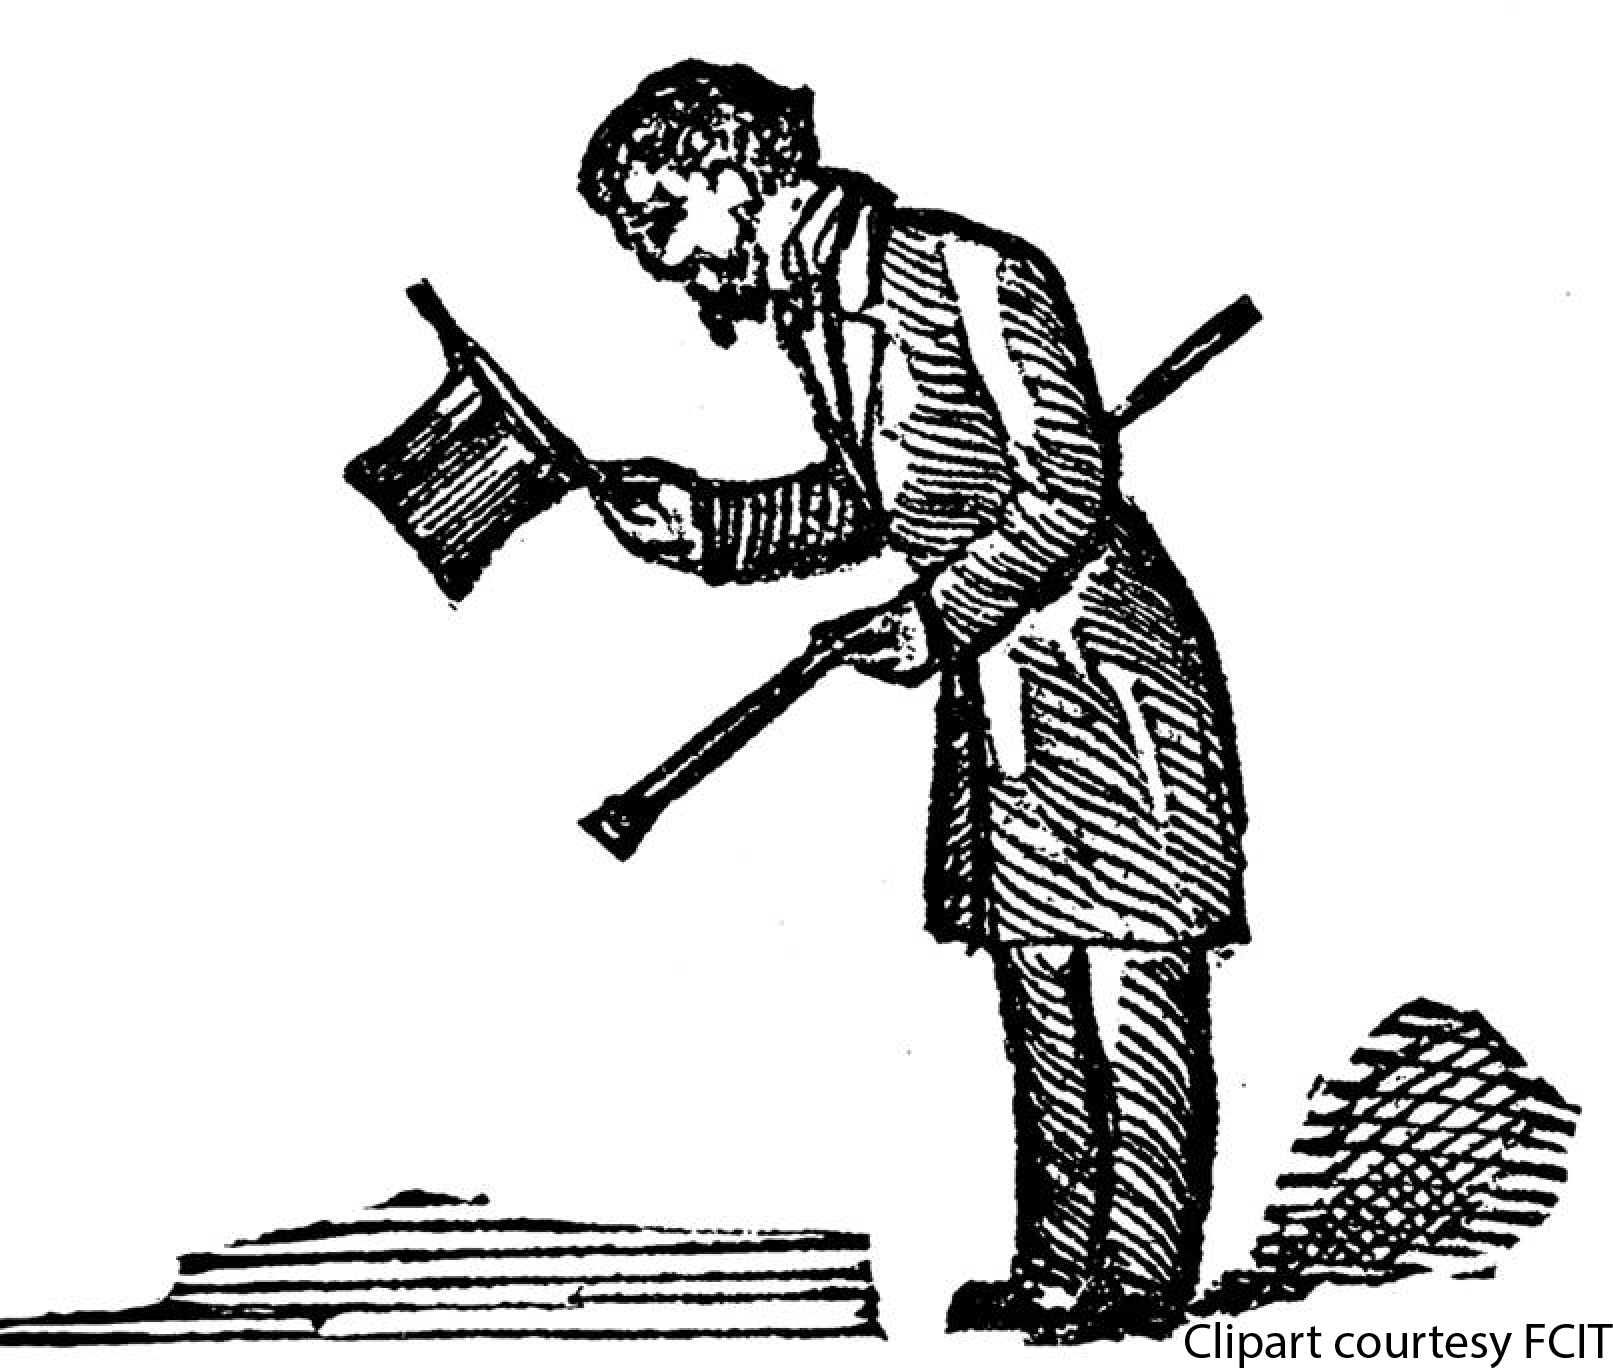
\includegraphics[width=0.5\textwidth]{figures/final}
	\end{figure}
	\begin{Large}
		\begin{center}
			\textbf{Any questions?}
		\end{center}
	\end{Large}	
\end{frame}



}
\end{document}

